\def\year{2021}\relax
%File: formatting-instructions-latex-2021.tex
%release 2021.1
\documentclass[letterpaper]{article} % DO NOT CHANGE THIS
\usepackage{aaai21}  % DO NOT CHANGE THIS
\usepackage{times}  % DO NOT CHANGE THIS
\usepackage{helvet} % DO NOT CHANGE THIS
\usepackage{courier}  % DO NOT CHANGE THIS
\usepackage[hyphens]{url}  % DO NOT CHANGE THIS
\usepackage{graphicx} % DO NOT CHANGE THIS
\urlstyle{rm} % DO NOT CHANGE THIS
\def\UrlFont{\rm}  % DO NOT CHANGE THIS
\usepackage{graphicx}  % DO NOT CHANGE THIS
\usepackage{natbib}  % DO NOT CHANGE THIS AND DO NOT ADD ANY OPTIONS TO IT
\usepackage{caption} % DO NOT CHANGE THIS AND DO NOT ADD ANY OPTIONS TO IT
\frenchspacing  % DO NOT CHANGE THIS
\setlength{\pdfpagewidth}{8.5in}  % DO NOT CHANGE THIS
\setlength{\pdfpageheight}{11in}  % DO NOT CHANGE THIS
%\nocopyright
%PDF Info Is REQUIRED.
% For /Author, add all authors within the parentheses, separated by commas. No accents or commands.
% For /Title, add Title in Mixed Case. No accents or commands. Retain the parentheses.
\pdfinfo{
/Title (AAAI Press Formatting Instructions for Authors Using LaTeX -- A Guide)
/Author (AAAI Press Staff, Pater Patel Schneider, Sunil Issar, J. Scott Penberthy, George Ferguson, Hans Guesgen, Francisco Cruz, Marc Pujol-Gonzalez)
/TemplateVersion (2021.1)
} %Leave this
% /Title ()
% Put your actual complete title (no codes, scripts, shortcuts, or LaTeX commands) within the parentheses in mixed case
% Leave the space between \Title and the beginning parenthesis alone
% /Author ()
% Put your actual complete list of authors (no codes, scripts, shortcuts, or LaTeX commands) within the parentheses in mixed case.
% Each author should be only by a comma. If the name contains accents, remove them. If there are any LaTeX commands,
% remove them.

\setcounter{secnumdepth}{2} 
\usepackage{paralist}
\usepackage[switch]{lineno}

% fig
\usepackage{subfig}
\usepackage{floatrow}
\usepackage[export]{adjustbox}


% math
\usepackage{amssymb}
\usepackage{amsmath}
\renewcommand{\Bbb}{\mathbb}
\DeclareMathOperator*{\cum}{\Box}

% algorithm2e
\usepackage[vlined, ruled, boxed,linesnumbered]{algorithm2e}
\SetKwInOut{Input}{Input}
\SetKwInOut{Output}{Output}
\SetKwInOut{Parameters}{Params}
\SetKwBlock{Setup}{Setup}{}
\SetKwFor{Loop}{Loop}{}


% defs
\usepackage[utf8]{inputenc}
\usepackage[english]{babel}
\usepackage{amsthm}
\theoremstyle{definition}
\newtheorem{definition}{Definition}
\newtheorem*{definition*}{Definition}
\newtheorem{example}{Example}
\newtheorem{lemma}{Lemma}
\newtheorem{theorem}{Theorem}
\newtheorem{corollary}{Corollary}

% tables
\usepackage{multirow}
\usepackage{array}
\usepackage{makecell}
\usepackage{hhline}
\usepackage{booktabs}

% macors
\newcommand{\norm}[1]{\left\lVert#1\right\rVert}
\newcommand{\reals}{\mathbb{R}}
\newcommand{\nnreals}{\reals^{\ge 0}}




\begin{document}


\title{Scalable and Safe Multi-Agent Motion Planning with \\ Nonlinear Dynamics and Bounded Disturbances}

\author{
    Jingkai Chen\textsuperscript{\rm 1}, 
    Jiaoyang Li\textsuperscript{\rm 2}\protect\thanks{Jiaoyang Li performed the research during her visit at Monash University.}, 
    Chuchu Fan\textsuperscript{\rm 1}, 
    Brian C. Williams\textsuperscript{\rm 1}
    \\
}
\affiliations{
    \textsuperscript{\rm 1} Massachusetts Institute of Technology \\
    \textsuperscript{\rm 2} University of Southern California \\
    jkchen@csail.mit.edu, jiaoyanl@usc.edu, chuchu@mit.edu, williams@csail.mit.edu
}
\maketitle

% We present a scalable and effective multi-agent motion planner that enables a group of agents to move to their desired locations while avoiding collisions with obstacles and other agents. As navigating a single agent with high-dimensional nonlinear dynamics and disturbances in obstacle-rich environments is difficult, the problem becomes more challenging when multiple agents are considered. We address this problem by finding a piecewise linear path for each agent such that the actual trajectories following these paths are guaranteed to satisfy the reach-and-avoid requirement. Given a tracking controller and the system dynamics, we pre-compute the tracking error bound between the actual trajectory of the closed-loop system and the minimum duration of each path segment. Using these bounds, we find a collision-free path for each agent by solving Mixed Discrete-Continuous Linear Programs and coordinate agents by using priority-based search. We demonstrate our method by benchmarking in 2D and 3D scenarios with ground vehicles and quadrotors, respectively, and show improvements over the solving time and the solution quality compared to two state-of-the-art multi-agent motion planners.

\begin{abstract}
We present a scalable and effective multi-agent safe motion planner that enables a group of agents to move to their desired locations while avoiding collisions with obstacles and other agents, with the presence of rich obstacles, high-dimensional, nonlinear, nonholonomic dynamics, actuation limits, and disturbances. We address this problem by finding a piecewise linear path for each agent such that the actual trajectories following these paths are guaranteed to satisfy the reach-and-avoid requirement. We show that the spatial tracking error of the actual trajectories of the controlled agents can be pre-computed for any qualified path that considers the minimum duration of each path segment due to actuation limits. Using these bounds, we find a collision-free path for each agent by solving Mixed Integer-Linear Programs and coordinate agents by using the priority-based search. We demonstrate our method by benchmarking in 2D and 3D scenarios with ground vehicles and quadrotors, respectively, and show improvements over the solving time and the solution quality compared to two state-of-the-art multi-agent motion planners.
\end{abstract}

\section{Introduction}

Multi-agent motion planning has a wide range of real-world applications, but it is notoriously difficult. Even navigating a single robot from an initial location to a goal location while avoiding collisions with obstacles is terribly challenging with the presence of rich obstacles, high-dimensional state space, nonlinear, nonholonomic dynamics, actuation limits, and disturbances. Not to say that when such complex robotic systems can interfere with each other in a shared environment, the scale of this problem is beyond the capability of most existing methods.

% play an important role in many real-world applications such as warehouse management, airport surface operations, and search-and-rescue to reduce operational costs and improve productivity. In these tasks, robots need to navigate from initial locations to goal locations while avoiding collisions with obstacles or other robots. 

% Navigating single robots such as ground vehicles and quadrotors is difficult with the presence of high-dimensional nonlinear dynamics and disturbances in obstacle-rich environments. While their motions are governed by the underlying dynamics in terms of positions, orientations, and velocities, their accelerations and steering rates are constrained by the controller capacities. This navigating problem becomes more challenging when the plans of robots can interfere with each other in a shared environment.

In this paper, we present \underline{S}calable and \underline{S}afe \underline{M}ulti-agent \underline{M}otion (S2M2) planner, a novel multi-agent motion planner that can fast and effectively generate provably safe plans for agent models with high-dimensional nonlinear dynamics and bounded disturbances in continuous time and space. Instead of directly planning dynamically-feasible trajectories, which are extremely computationally expensive, S2M2 exploits a separation-of-concerns approach: We first design piecewise linear (PWL) paths $S_i$ for each dynamical agent $\mathcal{A}_i$ to follow, with the understanding that the agents cannot follow those PWL paths exactly. However, we show that with appropriate tracking controllers, the actual trajectories of each agent under disturbances can converge to $S_i$ with guaranteed bounds on the spatial tracking error. More importantly, we show that such error bound can be pre-computed for any qualified PWL path. The secrete sauce behind the high efficiency of S2M2 is that we are able to formulate the problem of finding PWL paths for a single agent as a Mixed Integer-Linear Program (MILP), which can be solved efficiently using off-the-shelf MILP solvers.

To avoid inter-agent collisions, we wrap our single-agent motion planner with the priority-based search~\cite{ma2019searching} that explores the space of priority orderings using systematic search. When priorities are specified, lower-priority agents replan their paths while treating higher-priority agents as moving obstacles. Together with the MILP-based path planner and guaranteed tracking controller, S2M2 can efficiently find plans that are provably safe and robust to disturbances during execution. Moreover, by planning paths for multiple agents on a continuous map over continuous time, our method finds high-quality solutions with low flowtime (i.e., makespan sum of all single-agent plans).

% As planning dynamically-feasible trajectories directly is extremely computationally expensive, we tackle the dynamics by using a reference tracking framework, in which a tracking controller drives the agents to follow piecewise linear (PWL) paths. Thus, the task is then to find a path for each agent such that the actual trajectory is provable to satisfy the reach-and-avoid requirement (i.e., reaching the goal location while avoiding collisions with obstacles and other agents). We first pre-compute the requirements for the paths to be valid using reachability analysis \cite{sibai2020multi} and then solve a Mixed Integer-Linear Program (MILP) encoding to find such a valid path for each agent. To avoid inter-agent collisions, we wrap our single-agent motion planner with priority-based search \cite{ma2019searching} that explores the space of priority orderings using systematic search. When priorities are specified, lower-priority agents replan their paths while treating higher-priority agents as moving obstacles.

% The efficiency of our method is obtained by (a) using an efficient MILP-based trajectory planning method to find a PWL path for each agent, and (b) adopting the priority-based search to provide on-demand coordination. As our method considers the controller capacity against the disturbance and high-fidelity agent dynamics during planning, the obtained plans are provably safe and robust during execution. By directly planning and coordinating trajectories for multiple agents on a continuous map over continuous time, our method also finds high-quality solutions with low flowtime (i.e., makespan sum of all single-agent plans).


Consider an example of two disc-shaped vehicles making u-turns, as shown in Figure~\ref{fig:uturn}. Given the partially known initial locations and bounded disturbances, we first compute the spatial error bound of tracking a path segment, which is a line, and then consider this error together with the agent shape to obtain the possible swept area of the path segment. The swept area of agent $\mathcal{A}_1$ during its second segment $(p_{12}, p_{13})$ is shown in light blue. We also consider the minimum duration for each segment such that the agent has enough time to adjust its position after turning, which is $3$ seconds in our example. When our single-agent motion planner plans such paths for the agents, the obstacles are bloated with respect to the spatial tracking error and the agent shape, as shown in light red. 
%As long as the planned segments are away from these bloated obstacles, the agents will not sweep the obstacles. 
The planner also constrains each segment to respect the minimum segment duration. As we can see, when passing the corridor, both agents slow down and use this $3$ seconds to adjust their trajectories. After passing the corridor, agent $\mathcal{A}_2$ uses its full speed to approach its goal location. When potential collisions are detected, some agents are assigned higher priorities and thus are treated as moving obstacles for others. In our example, agent $\mathcal{A}_1$ is assigned higher priority and thus passes the corridor before agent $\mathcal{A}_2$.
%agent $\mathcal{A}_2$ waits for agent $\mathcal{A}_1$ to pass the corridor and then passes it to avoid collisions.


\begin{figure}[t]
    \vspace{4pt}
    \centering
    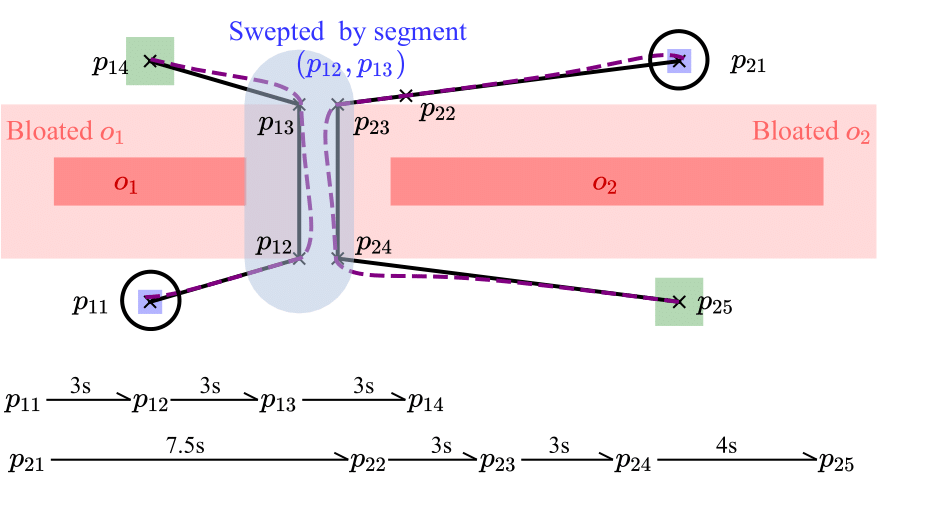
\includegraphics[width=0.99\columnwidth]{uturn.png}
    \caption{Example of two disc-shaped vehicles making u-turns. The initial and goal position sets are in blue and green, respectively. The obstacles are in red. The bloated obstacles are in light red. The paths of agents $\mathcal{A}_1$ and $\mathcal{A}_2$ are shown in solid black lines, and examples of their actual trajectories are shown in dashed purple lines. The swept area of agent $\mathcal{A}_1$ during its second segment is in light blue.}
    \label{fig:uturn}
\end{figure}

We compare the performance of S2M2 with ECBS-CT \cite{cohen2019optimal} and MAPF/C+POST \cite{honig2018trajectory} on 2D and 3D scenarios with ground vehicles and quadrotors, respectively. Results show that S2M2 outperforms both planners in terms of solution qualities with $15\sim70\%$ reduction for most instances. Moreover, S2M2 requires several magnitudes less time on pre-processing and also shows competitive runtime performance compared to the other two planners. 

% The remainder of this paper is organized as follows. We first summarize the related work in Section~\ref{section:related}. We describe the formal definition of our multi-agent motion planning problem and the necessary preliminaries in Section~\ref{section:formulation}. In Section~\ref{section:approach}, we introduce our method of pre-computing the tracking error and duration requirement over paths. Then, we introduce the MILP encoding to plan individual paths and our overall priority-based coordination approach. In Section~\ref{section:results}, we benchmark our approach on 2D and 3D scenarios with ground vehicles and quadrotors, respectively.


\section{Related Work}\label{section:related}

Many works have approached the Multi-agent Motion Planning (MAMP) problem from the perspectives of AI or robotics. These works can be generally divided into two categories with discrete and continuous settings, respectively. In the discrete setting, time and space are discretized into time steps and grids, respectively. Each agent occupies exactly one grid and can only move to adjacent grids at each time step. This problem is known as Multi-agent Path Finding (MAPF)~\cite{SternSoCS19}.
Researchers in the past years have made substantial progress in finding high-quality solutions to various scenarios with hundreds of agents and high congestion
as described in surveys \cite{MaWOMAPF16,felner2017search}. 
%These methods include reduction-based algorithms \cite{yu2013planning,erdem2013general,surynek2016efficient,bartak2017scheduling}, A*-based algorithms \cite{standley2010finding,wagner2011m,goldenberg2014enhanced}, and dedicated search algorithms \cite{sharon2013increasing,sharon2015conflict,barer2014suboptimal}. 
Prioritized planning is a popular and widely-used class of MAPF algorithms that coordinate multiple agents by specifying priorities among agents and forcing lower-priority agents to avoid collisions with higher-priority agents by treating their paths as dynamic obstacles \cite{velagapudi2010decentralized,vcap2015complete}. The most recent prioritized planning algorithm Priority-based Search (PBS) \cite{ma2019searching} systematically explores the space of priority orderings, which can lead to near-optimal solutions and possibly scale to a thousand agents. Our method adapts PBS to a continuous setting and thus can efficiently coordinate a large number of agents.

While the classical MAPF assumes synchronized and discretized time, zero-volume shapes, constant velocities, and rectilinear movements, several notable attempts have been made towards closing the gap between the classical MAPF and MAMP using more realistic models. This includes considering the continuous timeline, different-size agent shapes, kinematic constraints, robustness, and any-angle moving directions \cite{walker2018extended,li2019multi,cohen2019optimal,AndreychukYAS19,MaAAAI17,AtzmonAI20,YakovlevA17}. To obtain robust, executable, and high-quality solutions, our method also supports these features.

In the continuous setting, sampling-based motion planners are often used \cite{le2018cooperative,honig2018trajectory}. They first generate a probabilistic roadmap and then apply MAPF algorithms to it. These MAPF solutions are either used to guide the motion tree expansion \cite{le2018cooperative} or post-process to valid continuous trajectories \cite{honig2018trajectory}. Similar to our approach, these algorithms can handle high-order, nonlinear dynamics, and arbitrary complex geometries. Some optimization-based planners tend to solve a large optimization problem in which the decision variables define the trajectories for all agents \cite{augugliaro2012generation,mellinger2012mixed}, which are only demonstrated on small agent teams. %Our motion planner also uses optimization problems, but only for generating PWL paths for single agents, since the actual dynamically-feasible trajectories are obtained by tracking controllers and the inter-agent collisions are resolved on demand by PBS. As a result, our method can scale better than them while still producing high-quality solutions.
Our motion planner also uses optimization problems for generating trajectories. However, we only coordinate different agents on demand. To find a feasible plan for each agent, we focus on finding a PWL path satisfying certain duration and boundary requirements, which are encoded as MILPs and solved efficiently.
%To find a feasible plan for each agent, we focus on finding a PWL path satisfying certain duration and boundary requirements, which are encoded as MILPs and solved efficiently.


As a safety guarantee is important to successful execution, safe motion planning is receiving more attention recently. Several approaches are studied in a reference tracking framework, which uses the idea of bounding tracking errors through pre-computation based reachability analysis \cite{herbert2017fastrack,singh2017robust,vaskov2019towards,fan2020fast,majumdar2017funnel}. Other safe motion planners employ barrier functions \cite{barry2012safety,agrawal2017discrete} or use robust model predictive control with chance constraints \cite{blackmore2011chance,jasour2019sequential,yu2013tube}. Some of these works have been extended to the multi-robot setting \cite{wang2016safety,panagou2013multi,srinivasan2018control,desai2019soter,abs-1811-09914,richards2004decentralized}. %Recent learning-based methods also show great potential to effectively navigate robot teams \cite{semnani2020multi,liu2020mapper}. However, they cannot provide safety guarantees and may lead to collisions.

\section{Preliminaries and Problem Statement}\label{section:formulation}

For an $n$-dimensional vector $x \in \mathbb{R}^n$, $x^{(i)}$ is its $i^\text{th}$ entry, $\norm{x}$ is its Euclidean norm, and $B_\epsilon(x) \equiv \{y \in \mathbb{R}^n \|\ \norm{y-x} \leq \epsilon\}$ is the $\epsilon$-ball centered at $x$ with $\epsilon>0$. Given a matrix $H \in \mathbb{R}^{n \times m}$ and a vector $b \in \mathbb{R}^n$, an $(H,b)$-polytope $\texttt{Poly}(H, b)$ is the set $\{x \in \mathbb{R}^m \|\ Hx \leq b\}$. Each row of the polytope defines a halfspace $H^{(i)}x \leq b^{(i)}$, and each face is defined by $H^{(i)}x = b^{(i)}$. $\texttt{dP}(H)$ is the number of its faces.

\begin{definition}[Agent Model]
An agent model $\mathcal{A}_i = \langle  \mathcal{X}_i, \mathcal{U}_i, \mathcal{D}_i, f_i, \mathcal{P}_i\rangle$ is defined by its state space $\mathcal{X}_i \in \mathbb{R}^n$, input space $\mathcal{U}_i \subseteq \mathbb{R}^m$, disturbance space $\mathcal{D}_i \in \mathbb{R}^{l}$, dynamic function $f_i: \mathcal{X}_i \times \mathcal{U}_i \times \mathcal{D}_i \rightarrow \mathcal{X}_i$, and geometric shape $\mathcal{P}_i: \mathcal{X}_i \rightarrow 2^{\mathbb{R}^\delta}$.\footnote{A state is usually made up of positions, orientations, and velocities while an input refers to the input of the controller, such as accelerations and steering rates.}
\end{definition}

The semantics of agent dynamics are defined by trajectories, which describe the evolution of states over time. An input trajectory $u$ over duration $T$ is a continuous function $u$: $[0, T] \rightarrow \mathcal{U}_i$, which maps each time $t \in [0, T]$ to a control signal $u(t) \in \mathcal{U}_i$. Similarly, a disturbance trajectory $d$ over duration $T$ is a continuous function $d$: $[0, T] \rightarrow \mathcal{D}_i$. Given an input trajectory $u$ over $\mathcal{U}_i$, a disturbance trajectory $d$ over $\mathcal{D}_i$, and an initial state $x_{0} \in \mathcal{X}_i$, its state trajectory $\xi_i$ satisfies $\xi_i(x_0, u, d, 0) = x_{0}$ and for all $t > 0$,
\[\small
    \dot \xi_i (x_0, u, d, t) = f_i(\xi_i(x_0, u, d, t), u(t), d(t)).
\]

\begin{example}\label{example:model}
Consider a nonholonomic differential two-wheeled vehicle \cite{rodriguez2014trajectory} as an example. Its state $\xi_i(t)$ consists of three components: $p(t) = [p_x(t), p_y(t)]^T$ is the Cartesian coordinate of the center of inertia, $\theta(t)$ is the angular orientation, and $v(t)$ is the linear velocity. 
We also consider the bounded disturbances $d_x$ on $p_x$, $d_y$ on $p_y$, and $d_\theta$ on $\theta$.
The dynamic function $f_i$ consists of five components: $\dot p_x(t) = v(t) \cos \theta + d_x(t)$, $\dot p_y(t) = v(t) \sin \theta + d_y(t)$, $\dot v(t) = u_1(t) - k v(t)$, $\dot \omega(t) = u_2(t) - k \omega(t)$, and $\dot \theta(t) = \omega(t) + d_\theta(t)$,
%The dynamic function $f_i$ is as follows:
%\begin{equation}\small
%    \begin{aligned}
%    \dot p_x(t) = v(t) \cos \theta + d_x(t), \ 
%    \dot p_y(t) = v(t) \sin \theta + d_y(t), \\ 
    % \dot v(t) = \frac{1}{\rho m}(\tau_R(t) + \tau_L(t)), 
    % \dot \omega(t) = \frac{1}{\rho J}(\tau_R(t) - \tau_L(t)),\\
%    \dot v(t) = u_1(t) - k v(t),  \
%    \dot \omega(t) = u_2(t) - k \omega(t),\\
%    \dot \theta(t) = \omega(t) + d_\theta(t), \\
%    \end{aligned}
%\end{equation}
where $k$ is a constant, and $u_1(t)$ and $u_2(t)$ are control force and torque as inputs, which can be used to compute the torques for the left and right wheels.
%$\rho$ is the wheel radius, $l$ is the distance between both wheels, and $m$ and $J$ are the mass and moment of inertia, respectively.
\end{example}

\begin{definition}[MAMP]
A multi-agent motion planning (MAMP) problem is defined by
$\langle \mathcal{W}, O, \mathcal{A},\mathcal{X}^\texttt{init}, \mathcal{X}^\texttt{goal} \rangle \nonumber$, where workspace $\mathcal{W} \subseteq \mathbb{R}^\delta$ is a bounding box in $\mathbb{R}^\delta$; $\delta=2$ for ground vehicles and $\delta = 3$ for aerial and underwater vehicles, and $\xi_i(t) \downarrow \mathcal{W}$ is the projection of $\xi_i(t)$ to the workspace; obstacles $O = \{o_i\}_i \subseteq \mathcal{W}$ are polytopes in $\mathcal{W}$; $\mathcal{A} = \{\mathcal{A}_1,..,\mathcal{A}_N\}$ is a set of agent models; $\mathcal{X}^{\texttt{init}}_i \subseteq \mathcal{X}_i $ and $\mathcal{X}^{\texttt{goal}}_i \subseteq \mathcal{X}_i$ are the initial set and the goal set of  $\mathcal{A}_i$.
The planning problem is to find inputs  $(u_1,..,u_N)$ for every $(x^\texttt{init}_1,..,x^\texttt{init}_N) \in \mathcal{X}^{\texttt{init}}_1  \times \cdots \mathcal{X}^{\texttt{init}}_N$ and every disturbance trajectories $(d_1,..,d_N)$ such that the state trajectories $(\xi_1,..,\xi_N)$ satisfy the
reach-and-avoid requirement: 
\begin{enumerate}
    \item (Dynamics) $\forall \mathcal{A}_i \in \mathcal{A}$, $\xi_i(t) \equiv \xi_i(x^\texttt{init}_i,u_i,d_i,t)$;
    \item (Reach goal set) $\exists t \geq 0$, $\forall \mathcal{A}_i \in \mathcal{A}$, $\xi_i(t) \in \mathcal{X}_{i}^\texttt{goal}$;
    \item (Avoid obstacles) $\forall t \geq 0$, $\forall \mathcal{A}_i \in \mathcal{A}$,  $\mathcal{P}_i(\xi_i(t)) \in \mathcal{W}$ and $\mathcal{P}_i(\xi_i(t)) \cap O = \emptyset$.
    \item (Avoid inter-agent collisions) $\forall t \geq 0$, $\forall \mathcal{A}_i, \mathcal{A}_j \in \mathcal{A}$ and $i \not = j$,   $\mathcal{P}_i(\xi_i(t)) \cap \mathcal{P}_j(\xi_j(t)) = \emptyset$
\end{enumerate}
\end{definition}

In this work, we will solve the MAMP problem by finding a  piecewise linear (PWL) path for each agent. The PWL paths for the agents will be sufficiently far away from the obstacles and from each other so that agents' tracking controllers can drive them to follow their PWL paths to reach their goals without collisions. Here we define PWL paths, tracking controllers, and reachability envelopes of each agent with a given tracking controller.

\begin{definition}[Piecewise Linear Path]
A PWL path $S_i$ in the workspace $\mathcal{W}$ for an agent $\mathcal{A}_i$ is a function $S_i: \nnreals \rightarrow \mathcal{W}$ that maps a time point to a position $S_i(t) \in \mathcal{W}$, which can be constructed from a sequence of time-stamped waypoints $S_i= \texttt{Path} ( \{(t_k, p_k)\}_k)$ such that $S_i(t) = p_{k-1} + \frac{p_k - p_{k-1}}{t_k - t_{k-1}} (t - t_{k-1})$ for $t\in[t_{k-1},t_{k}]$. $(t_k, p_k) \in \nnreals \times \mathcal{W}$ is called the $k^\text{th}$ waypoint of path $S_i$, and $S_i(t)$ when $t\in[t_{k-1},t_{k}]$ is called the $k^\text{th}$ segment of $S_i$ and denoted by $S^{(k)}_i$. %A PWL path $S$ is differentiable except for the waypoints $\{(t_k, p_k)\}_k$.
\end{definition}


\begin{definition}[Decentralized Tracking Controller]
A tracking controller for an agent $\mathcal{A}_i$ is a (state feedback) function $g_i: \mathcal{X}_i \times \mathcal{W} \rightarrow \mathcal{U}_i$. At any time $t$, a tracking controller takes in  a current state of the system $x \in \mathcal{X}_i$ and a desired position $S_i(t) \in \mathcal{W}$, and gives an input $g_i(x, S_i(t)) \in \mathcal{U}_i$ for $\mathcal{A}_i$.
\end{definition}

Fix a tracking controller $g_i$ and a PWL path $S_i$ for an agent $\mathcal{A}_i$, the resulting closed-loop controlled agent becomes an {\em autonomous system}. We use  $\xi^{g_i}_i(x_0, S_i, d_i, t)=\xi_i(x_0, g_i(x_0, S_i(t)), d_i, t)$ to represent the trajectory of the controlled agent $\mathcal{A}_i$ starting from $x_0$ with disturbance $d_i$. The {\em reachablity envelope} of a controlled agent is a set of states around the PWL path that contains all possible actual trajectories of the controlled agent, defined as follows.
% , an initial state $x_0 \in \mathcal{X}^\texttt{init}_i$, and a disturbance trajectory $d_i$, the resulting trajectory $\xi_i^g$ of the closed control system satisfies $\xi^g_i(t)(x_0, g_i, S_i d_i, 0) = 0$ and for all $t>0$:
% \begin{equation}
%     \dot \xi^g_i(x_0, g_i, S_i, d_i, t) = f(\xi^g_i(t), g_i(\xi^g_i(t), S_i(t)), d_i(t))
% \end{equation}
\begin{definition}[Reachability Envelope]
    Given an agent model $\mathcal{A}_i = \langle  \mathcal{X}_i, \mathcal{U}_i, \mathcal{D}_i, f_i, \mathcal{P}_i\rangle$, an initial set $\mathcal{X}^\texttt{init}_i \subseteq \mathcal{X}_i$, a PWL path $S_i$, and a tracking controller $g_i$, the reachablity envelope  at time $t$ is %\texttt{Reach}(\mathcal{X}^\texttt{init}_i,S_i, g_i,  D_i,  t)$ as 
    $\texttt{Reach}_{\mathcal{A}_i}(\mathcal{X}^\texttt{init}_i,S_i, g_i,  D_i,  t) = 
    \{ \xi^{g_i}_i(x_0,  S_i, d_i, t) \in \mathcal{X}_i \,|\, \exists x_0 \in \mathcal{X}^\texttt{init}_i, \exists d_i: \nnreals \rightarrow \mathcal{D}_i \}$.
    %\begin{equation}\small
    %\begin{aligned}
    %&\texttt{Reach}_{\mathcal{A}_i}(\mathcal{X}^\texttt{init}_i,S_i, g_i,  D_i,  t) = \\
    %& \{ \xi^{g_i}_i(x_0,  S_i, d_i, t) \in \mathcal{X}_i \,|\, \exists x_0 \in \mathcal{X}^\texttt{init}_i, \exists d_i: \nnreals \rightarrow \mathcal{D}_i \}.
    %\end{aligned}    
    %\end{equation}
\end{definition}

\begin{example}\label{example:controller}
Let a $S(t) = [p^*_x(t), p^*_y(t)]^{T}$ be a PWL path of waypoint sequence $\{(t_k, p_k)\}_k$. From~\cite{rodriguez2014trajectory}, a valid tracking trajectory for Example~\ref{example:model} can be constructed as 
\[\small
\begin{bmatrix}
u_1\\
u_2
\end{bmatrix}=
\begin{bmatrix}
\cos \theta & \sin \theta \\
-\sin \theta/L & \cos \theta/L 
\end{bmatrix}
\begin{bmatrix}
u_1^\prime + v \omega \sin \theta + L \omega^2 \cos \theta \\
u_2^\prime - v \omega \cos \theta + L \omega^2 \sin \theta
\end{bmatrix}
,
\]
where $L$ is a positive constant and $u_1^\prime, u_2^\prime$ are computed as
\[\small
\begin{bmatrix}
u_1^\prime\\
u_2^\prime
\end{bmatrix}=
\begin{bmatrix}
v^* \cos \theta^* - L \sin \theta^* \omega^*\\
v^* \sin \theta^* + L \cos \theta^* \omega^*
\end{bmatrix} +
G\frac{z^{2p-1}}
{1+\|z\|^{2p-1}},
\]
where $G$ is a positive constant, $p$ is a positive integer, {\small$z = \begin{bmatrix}
(p_x - p_x^*) + L (\cos \theta - \cos \theta^*)\\
(p_y - p_y^*) + L (\sin \theta - \sin \theta^*)
\end{bmatrix}$} and $\forall t \in [t_{k-1},t_k], v^*(t) = \frac{\|p_k - p_{k-1}\|}{t_k - t_{k-1}}, \theta^*(t) = \mbox{atan2}(p_{k}-p_{k-1})$.
The dashed purple lines in Figure~\ref{fig:uturn} illustrate such two trajectories of the closed-loop agents.
\end{example}



\section{Approach}\label{section:approach}
Figure~\ref{fig:diagram} gives an overview of our approach S2M2, consisting of three key modules: 
\begin{inparaenum}
    \item[(a).] (Figure~\ref{fig:diagram} left): Given a tracking controller $g_i$ for each agent $\mathcal{A}_i$, pre-compute reachability envelopes for any PWL path $S_i$ using symmetry transformations and cashed reachability envelopes, to get two key parameters: (1) an upper bound of the spatial tracking error between the actual trajectory $\xi_i^{g_i}(x_0, S_i, d_i, t) \downarrow \mathcal{W}$ and $S_i$, and (2) the minimum duration of each path segment $S_i^{(k)}$ such that the spatial tracking error bound is always valid (Section \ref{section:approach:reachability}). 
    \item[(b).]  (Figure~\ref{fig:diagram} middle): Given two parameters from (a), the safe motion planning problem for each agent is reduced to finding a PWL path that is sufficiently far from the obstacles and other agents, which is further encoded as a MILP problem (Section~\ref{section:approach:milp}).
    \item[(c).] (Figure~\ref{fig:diagram} middle): To coordinate multiple agents, employ priority-based search to avoid inter-robot collisions, in which some agents treat other agents as moving obstacles and replan their paths optimally (Section~\ref{section:approach:pbs}). 
\end{inparaenum}
Putting them all together (Figure~\ref{fig:diagram} right), S2M2 finds a PWL path for each agent in the multi-agent system, so the closed-loop agents driven by tracking controllers can move along the PWL paths to 
% Given a tracking controller and the system dynamics, S2M2 find PWL paths for all the agents such that their controllers can drive them along these paths to 
safely achieve the reach-and-avoid requirement. 

% A natural thought that has been extensively explored recently is to exploit a separation of concerns that exists in the problem: (A) how to design a reference (also called expected or nominal) trajectory $x^*(t)$ to drive a robot to its goal safely without any uncertainty or disturbance, and (B) how to 

% \begin{enumerate}
%     \item The reachability analysis module evaluates the tracking error performance of the controller with respect to the system dynamics. It computes two parameters, namely the spatial difference bound between the agent and the path at any time and the minimum duration of each path segment such that the spatial difference can be bounded.
%     \item Given these two parameters, S2M2 encodes the motion planning problem for each agent as a MILP, which finds a sequence of time-stamped waypoints as a PWL path. This path satisfies the duration constraint and is away from the obstacles with respect to the given spatial error. 
%     \item S2M2 employs priority-based search to coordinate inter-robot collisions, in which some agents treat other agents as moving obstacles and replan their paths optimally. 
% \end{enumerate}




% In the rest of this section, we introduce %how to compute the spatial different bound and the minimum duration requirements 
% the reachability analysis (Section \ref{section:approach:reachability}), the optimal single-agent motion planner (Section~\ref{section:approach:milp}), the moving obstacle encoding (Section~\ref{section:approach:moving}), and the priority-based coordination method (Section~\ref{section:approach:pbs}).
 
 
\begin{figure}[t]
\centering
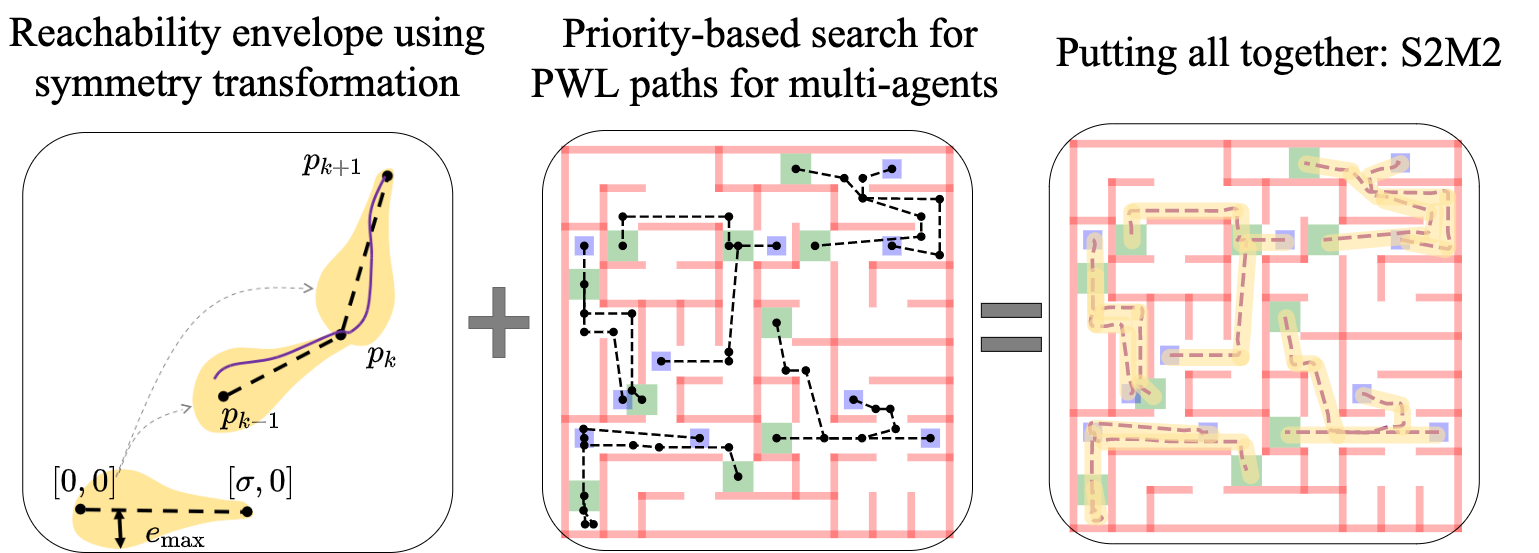
\includegraphics[width=0.99\columnwidth]{overview.png}
\caption{Schematic illustration of the approach.}
\label{fig:diagram}

\end{figure}

 


% \begin{algorithm}[t]
% \small
% \caption{S2M2}
% \label{alg:s2m2}
% \Input{MAMP instance $\langle \mathcal{W}, O, \mathcal{A},\mathcal{X}^\texttt{init}, \mathcal{X}^\texttt{goal} \rangle $ \\
%     Controller $g_i$ for every agent $\mathcal{A}_i \in \mathcal{A}$} 
% \Output{PWL Path $S_i$ for every agent $\mathcal{A}_i \in \mathcal{A}$}

% \For{$\mathcal{A}_i \in \mathcal{A}$}{$(e_{i, \text{max}}, T_{i,\text{min}}, T_{i,\text{min}}') \gets \text{analysis  } \mathcal{A}_i \text{ given } g_i $ }
% $\text{Individually plan PWL paths } S \text{ and initialize prioity tree}$ \;
% \For{\upshape $N \gets \text{ next node in the priroity tree}$ }
% {
%  \lIf{\upshape $N.S$ is collision free}{\KwRet{$S$}}
%  $\mathcal{A}_i \gets \text{agent that needs replan in } N$\;
%  Encode higher-priority agents in $N$ as obstacles $O'$\;
%  Update $N.S_i$ by replanning $\mathcal{A}_i$ in $\mathcal{W}$ from $\mathcal{X}^\texttt{init}_i$ to $ \mathcal{X}^\texttt{goal}_i $ while avoiding $O, O' $ wrt $e_{i, \text{max}}, T_{i,\text{min}}, T_{i,\text{min}}'$\;
% }

% \end{algorithm}

 
 

\subsection{Computing Reachability Envelopes}\label{section:approach:reachability}

% The key idea behind the use of the PWL path is that the reachability envelope of following PWL paths can be pre-computed independent of the concrete values of the waypoints and time stamps.
Beyond the fact that a PWL path can be computed efficiently through solving a MILP problem (see Section~\ref{section:approach:milp}), another key idea behind the use of PWL paths is that the reachability envelopes can be pre-computed independent of the concrete values of the PWL paths' waypoints. In this way, we pre-compute the following two parameters of these envelopes, which are used as constraints in finding the PWL paths: (1) an upper-bound of the distance between the actual trajectory projected to the workspace and the reference PWL path; and (2) the minimum duration bound for each path segment to guarantee such distance bound.
% In this way, we know in advance how far the actual trajectories of each agent are away from their reference PWL paths. Then as long as the PWL paths are sufficiently far from the obstacles and from each other, the actual trajectories are also collision-free. Therefore, we can reduce the motion planning problem to multi-agent waypoints synthesis problem, which will be solved in the following sections.

Various methods can be used to pre-compute reachability envelopes, including Contraction Metrics~\cite{singh2017robust,tsukamoto2020neural}, Lyapunov functions~\cite{fan2020fast}, Funnels~\cite{majumdar2017funnel}, and Hamilton-Jacobi analysis~\cite{herbert2017fastrack}.
In this section, we take an alternative approach called symmetry transformation. Symmetry transformations on dynamical systems are defined as the ability to compute new trajectories (reachable states) of the same dynamics by applying symmetry operators (e.g., translation and rotation) on existing trajectories (reachable states) \cite{russo2011symmetries}. We show that under mild assumptions, using symmetry transformation, the reachability envelope of an agent  following a PWL path can be constructed from a finite number of reachability envelopes. These envelopes are of the same agent following a single straight line along the x-axis defined by waypoints $(0,[0,0]^T)$ and $(T, [\sigma, 0]^T)$. Then, without knowing the waypoints of a PWL path, we can pre-compute these envelopes around the x-axis and extract the spatial error bound and the minimum segment duration from them.


For the rest of this section, we abuse the notation and use $\texttt{Reach}_{\mathcal{A}_i}^{g_i}(\mathcal{X}^\texttt{init}_{i,k}, S_{i}^{(k)}, t)$ to denote the reachability envelope of agent $\mathcal{A}_i$ following path segment $ S_{i}^{(k)}$ from initial set $\mathcal{X}^\texttt{init}_{i,k}$ at time $t_{k-1}$. The initial set is defined recursively as $\mathcal{X}^\texttt{init}_{i,k}$ $=\texttt{Reach}_{\mathcal{A}_i}^{g_i}(\mathcal{X}^\texttt{init}_{i,(k-1)}, S_{i}^{(k-1)}, t_{k-1})$.
%The following definitions are taken from \cite{russo2011symmetries} modified for systems with inputs instead of autonomous systems of the form $\dot{x} = f(x)$.

% In what follows, we abuse the notation and use $f_{g_i}(x, \{(t_{k-1},p_{k-1}), (t_k, p_k)\}, d)$ to denote the dynamics, and $\xi^{g_i}_i(x_0,\{(t_{k-1},p_{k-1}), (t_k, p_k)\},d,t)$ to denote the trajectory of the system following a line segment defined by connecting two time-stamped $(t_{k-1},p_{k-1})$ and $(t_k, p_k)$, where the trajectory starts from $x_0$ at time $t_{k-1}$.

% \begin{definition}[Adopted from~\cite{sibai2020multi}]
% 	\label{def:symmetry}
% 	Let $\Gamma$ be a group of linear operators acting on $\mathbb{R}^n$. We say that $\gamma \in \Gamma$ is a symmetry of an agent $\mathcal{A}_i$ if for any trajectory, $\xi^{g_i}_i(x_0,\{(t_{k-1},p_{k-1}), (t_k, p_k)\},d,t)$, $\gamma \cdot \xi^{g_i}_i(x_0,\{(t_{k-1},p_{k-1}), (t_k, p_k)\},d,t)$ is also a trajectory. Furthermore, the closed-loop dynamic function $f_{g_i}: \mathcal{X}_i \times (\nnreals \times \mathcal{W})^2 \times \mathcal{D}_i \rightarrow \mathcal{X}_i$ is said to be $\Gamma$-equivariant if for any $\gamma \in \Gamma$, there exists $\rho: (\nnreals \times \mathcal{W})^2 \rightarrow (\nnreals \times \mathcal{W})^2$ and $\eta: \mathcal{D}_i \rightarrow \mathcal{D}_i$ such that for all $\state \in \mathcal{X}_i$, $\frac{\partial \gamma}{\partial \state} f(\state, \{(t_{k-1},p_{k-1}), (t_k, p_k)\}, d) = f(\gamma(\state), \rho(\{(t_{k-1},p_{k-1}), (t_k, p_k)\}), \eta(d))$.
% \end{definition} 

% Using the symmetry operation $\gamma$, we can construct a new trajectory without simulating the system but instead by just transforming the entire old trajectory using $\gamma(\cdot)$.


% \begin{theorem}[Adopted from~\cite{sibai2020multi}]
% 	\label{thm:sol_transform_input_nonlinear}
% 	If $f_{g_i}$ is $\Gamma$-equivariant, then for any solution $\xi^{g_i}_i(x_0,\{(t_{k-1},p_{k-1}), (t_k, p_k)\},d,t)$ and $\gamma \in \Gamma$, $\gamma(\xi^{g_i}_i(x_0,\{(t_{k-1},p_{k-1}), (t_k, p_k)\},d,t)) = \xi(\gamma(\state_0),\rho(\{(t_{k-1},p_{k-1}), (t_k, p_k)\}), \eta(d), t)$, where $\rho$ and $\eta$ are the transformations associated with $\gamma$ in Definition~\ref{def:symmetry}.
% \end{theorem}

% Let us consider the robotic system in Example~\ref{example:model} with the tracking controller as in Example~\ref{example:controller} and a trajectory $\gamma(\xi^{g_i}_i(x_0,\{(t_{k-1},[0,0]^T), (t_k, [\|p_k - p_{k-1}\|, 0]^T)\},d,t))$, which follows a path from the origin along the $x$-axis.
% The following transformation can be proved to be a valid symmetry transformation to construct the trajectory following a path from $(t_{k-1},p_{k-1})$ to $(t_k, p_k)$ (detailed proof is provided in the supplementary material).
By using a symmetry operator $\gamma$ constructed by translation and rotation, the reachability envelopes of segment $ S_i^{(k)}$ can be constructed from that of segment  $S^{x\text{-axis}}_i$ with the same length and time duration, which is as follows:
\begin{equation*}\scriptsize
    \texttt{Reach}_{\mathcal{A}_i}^{g_i}(\mathcal{X}^k_i, S_i^{(k)},t) = 
    \gamma\left(  \texttt{Reach}_{\mathcal{A}_i}^{g_i} \left(\gamma^{-1}(\mathcal{X}^k_i), S^{x\text{-axis}}_i, t)\right)  \right),
\end{equation*}
where for a set $\mathcal{Y}\subseteq \mathcal{X}$,  $\gamma(\mathcal{Y}) = \{\gamma(x) \ | \ x \in \mathcal{Y}\}$ and $\gamma^{-1}(\mathcal{Y}) = \{ y \ |\ \exists x \in \mathcal{Y}, \gamma(y) = x\}$. 

Since the translation and rotation transformations preserve vector lengths, $\gamma \left(\texttt{Reach}(\cdot,\cdot,\cdot)\right)$ has the same size as  $\texttt{Reach}(\cdot,\cdot,\cdot)$.
% \jingkai{Prove error after $\gamma$ transformation does not change?}
Thus, as long as (1)  we pre-compute the reachability envelope that follows a path $S^{x\text{-axis}}_i$ from $\mathcal{X}^\texttt{init}_i$ with duration $T$ and length $\sigma$ for sufficiently long $T$ and all $\sigma \in [v_{\min}T, v_{\max}T ]$; and (2) $\gamma^{-1}(\mathcal{X}^k_i) \subseteq \mathcal{X}^\texttt{init}_i$ for all $k=\{1,..,K\}$ ($K$ is the number of path segments in $S_i$), we can always construct the reachability envelope of following PWL paths using the symmetry operator $\gamma$ on these pre-computed envelopes. These envelopes can be computed using any nonlinear reachability toolbox \cite{chen2013flow,Althoff2018b,fan2017d}. The reachability envelope construction for aerial vehicles or underwater vehicles is similar. 

To understand how far the reference path $S_i$ needs to be away from the obstacles, we define the maximum spatial tracking error $e_{i, \max}$ as follows:
\begin{equation*}\small
\begin{aligned}
&e_{i,\max} = \text{argmin}_{e}  \forall \sigma \in [v_{\min}T, v_{\max}T ], \forall t \in [0,T], \\ &B_{e}(S^{x\text{-axis}}_i(t)) \supseteq 
\texttt{Reach}_{\mathcal{A}_i}^{g_i} \left(\mathcal{X}^\texttt{init}_i, S^{x\text{-axis}}_i,  t\right) \downarrow \mathcal{W},
\end{aligned}
\end{equation*}
where $S^{x\text{-axis}}_i = \texttt{Path}(\{(0,[0,0]^T), (T, [\sigma, 0]^T) \})$.
% where $S(t))$ is the straight path connecting $(0,[0,0]^T)$ and $(T, [\sigma, 0]^T)$. 
We implement this equation by first discretizing $[v_{\min}T, v_{\max}T]$ with $\Delta$ and calculating the error bound $e$ for each reachability envelopes with length $\sigma_j = (v_{\min}T+j\Delta)$. Then, we choose the maximum value over all these errors as $e_{i,\texttt{max}}$.

To guarantee that, for any segment $S_i^{(k)}$, the trajectories can converge close enough to it before switching to the next segment, the tracking controller needs to be applied for a sufficiently long time. So we identify the minimum segment duration $T_{i,\min} $ such that $t_k - t_{k-1} > T_{i,\min}$ guarantees $\gamma^{-1}(\mathcal{X}^k_i) \subseteq \mathcal{X}^\texttt{init}_i$, for $k=1, \dots, K$.  Similarly, for the last line segment $S_i^{(K)}$, %$S_i^{(K)} = \texttt{Path}(\{(t_{K-1},p_{K-1}),(t_K, p_K)\})$, 
we also find the minimum duration $T_{i,\min}^\prime < t_{K} - t_{K-1} $ such that the final reachable states of the trajectory following path $ S_i^{(K)}$ have enough time to be sufficiently small to fit into the goal set $\mathcal{X}^\texttt{goal}_i$. 

Notice is that for agents with relatively larger actuation limits compared to their velocity ranges, the obtained $e_{i,\text{max}}$ and $T_{i,\min}^\prime$ will be smaller, and our planner will generate paths that are closer to obstacles and make turns more often to minimize the plan makespan. It is also of our users' choices to specify smaller accelerations when computing reachability envelopes, which leads to smoother trajectories but may result in over-conservative plans or even failures. In addition, we can restrict the velocity ranges to have smaller $e_{i,\text{max}}$ and $T_{i,\min}^\prime$, which mitigates the problem of being over-conservative but may lead to plans with longer makespans.


% We find the final error of a segment with duration $T$ as follows: 
% \begin{equation*}\small
% \begin{aligned}
% &e_\texttt{fl} = \text{argmin}_{e} \forall \sigma \in [v_{\min}T, v_{\max}T], \forall t\in[T_{\min}^{\prime}, T] \\
% &B_{e}( S^{x\text{-axis}}_i(t) \supseteq \texttt{Reach}_{\mathcal{A}_i} \left(\mathcal{X}^\texttt{init}_i, S^{x\text{-axis}}_i, g_i,  D_i,  t \right) \downarrow \mathcal{W}.
% \end{aligned}
% \end{equation*}

% \jingkai{I am thinking about: the minimum duration of the first segment and the last segment should be computed separately. For other segments, we need the end error to be smaller than the start error. However, this is different for the first and last segment: (1) the end error of the first segment should be smaller than the start error of other segments, but its start error is extracted from the initial error, which might be larger and take longer duration; (2) the start error of the last segment should be the start error of other segments, but its end error should respect the goal set, which might be smaller and take longer duration.}


% A state-input reference or a reference consists of a reference state trajectory (reference trajectory) $\xi_\text{ref}$ and a reference input trajectory (reference input) $u_\text{ref}$ such that the agent is expected to be at position $p_k$ when the time is $t_k$. A tracking controller for each agent can real-time compute inputs in a distributed fashion with respect to $(\xi_\text{ref}, u_\text{ref}$), and the resulting state trajectories are guaranteed to follow $S$ with a bounded error as long as the disturbances are bounded. A tracking controller is a function $g: \mathcal{X}_i \times \mathcal{X}_i \times \mathcal{U}_i \rightarrow \mathcal{U}_i$.  At any time $t$, a tracking controller takes in a current state of the system $x \in \mathcal{X}$, a reference state $\xi_\text{ref}(t)$, and a reference input $u_\text{ref}(t)$, and gives an input $g(x, \xi_\text{ref}(t), u_\text{ref}(t))$.




%Note that the commutativity condition with the vector field of the ODE in Definition~\ref{def:equivariance_input} is similar to the properties of Lyapunov functions in the sense that it proves a property about the solutions without inspecting them individually. 



\subsection{Finding Paths for Single Agents}\label{section:approach:milp}


In this section, we describe the method for finding a PWL path for a single agent $\mathcal{A}_i$ with the presence of static obstacles and moving obstacles. To obtain a valid path, we solve a MILP problem. The decision variables of this MILP are $(p_{0}, p_{1}, ..,p_{K})$ with domain $\mathcal{W}$ and $(t_{0}, t_{1}, .., t_{K})$ with domain $\nnreals$, which represent the waypoint positions and their time stamps, respectively. The objective is to minimize the makespan $t_{K}$. We constrain the initial position to be at the center of the initial set $S^\texttt{init}_i$ and the initial time to be $0$: %which is as follows
% \begin{equation}\small
    $(p_0 = \texttt{Center}(S^\texttt{init}_i \downarrow \mathcal{W})) \land ( t_0 = 0 )$.
% \end{equation}

In the rest of this section, we introduce the other sets of the constraints that ensure the instantiated trajectory of the obtained path is valid with respect to the system dynamics, spatial tracking error $e_{i,\texttt{max}}$, minimum segment duration $T_{i,\texttt{min}}$, and minimum duration for the last segment $T_{i,\texttt{min}}^\prime$.

\subsubsection{Time-Position Constraints}
We first add constraints over the duration $(t_k - t_{k-1})$ and the spatial difference $(p_k - p_{k-1})$ for each segment to make sure its velocity $\frac{p_k - p_{k-1}}{t_k - t_{k-1}}$ respects the velocity bound. 
% We denote the feasible set of $f \downarrow \mathcal{W}(q, u)$ as $\mathcal{U}_p$ and $\mathcal{U}_p = \{f \downarrow \mathcal{W}(q, u) \ | \ (p, q) \in \mathcal{X}, u \in \mathcal{U}  \}$. Consider a vehicle model with state $x = (p_x, p_y, \theta)$, position $(p_x, p_y)$, and input $(v, w)$. If the velocity $v$ should be no more than $1m/s$, and $f\downarrow \mathcal{W} = [v \cos(\theta), v \sin(\theta)]^T$, we know $f\downarrow \mathcal{W} \in \mathcal{U}_p = B_1(0)$. 
Let $v_\text{min}$ and $v_\text{max}$ be the minimum and maximum allowable velocities of the agent model, respectively. Then, the feasible velocity set is $B_\texttt{vmax}(0) / B_\texttt{vmin}(0)$. We further under-approximate $B_\texttt{vmax}(0)$ to polytope $\texttt{Poly}(H_\texttt{vmax}, b_\texttt{vmax})$, and over-approximate $B_\texttt{vmin}(0)$ to polytope $\texttt{Poly}(H_\texttt{vmin}, b_\texttt{vmin})$. The constraints to ensure each segment to satisfy such dynamic relations are:
\begin{equation*}\small 
    \begin{aligned}
     (\lor_{j=1}^{\texttt{dP}(H_\texttt{vmin})} H_\texttt{vmin}^{(j)}(p_k - p_{k-1}) \geq   b_\texttt{vmin}^{(j)}(t_k - t_{k-1})) \\
    \land (H_\texttt{vmax}(p_k - p_{k-1}) \leq   b_\texttt{vmax}(t_k - t_{k-1}))\
    \forall k = 1,2,..,K
    \end{aligned}
\end{equation*}

We handle disjunctive linear constraints $(\lor_{j=1}^{\texttt{dP}(H)} H^{(j)} x \leq b^{(j)}$ by using the big-M method. We define a $\texttt{dP}(H)$-vector of binary variables $\alpha$, and $\alpha^{(j)} = 1$ if and only if $H^{(j)} x \leq b^{(j)}$ holds for $x$. Let $M$ be a very large positive number, then the constraints is encoded as %and the implementation is as follows:
% \begin{equation}\small
%     \begin{aligned}
         $(\land_{j=1}^{\texttt{dP}(H)} H^{(j)} x + M(1 - \alpha^{(j)}) \leq b^{(j)}) \land (\sum_{j=1}^{\texttt{dP}(H)} \alpha^{(j)} \geq 1)$.
%     \end{aligned}
% \end{equation}

\subsubsection{Reach-and-Avoid Constraints}

As the actual tracking trajectories deviate from the PWL paths due to inertia, actuation limits, disturbances, and uncertain initial position, we should consider this deviation when encoding constraints related to obstacles and goals.  We have shown that the error between the actual trajectory and the PWL path can be bounded within $e_{i, \text{max}}$ for each agent $\mathcal{A}_i$. In addition to the position deviation, we should consider the agent shape, and the swept area should not intersect with obstacles as well. Then, we know all the possible swept area at position $p$ is $R = p \oplus B_{l}(0)$, where $l = e_{i, \text{max}} + r_i$, and $r_i$ is the radius of the ball containing agent $\mathcal{A}_i$. For obstacle $o = \texttt{Poly}(H_o,b_o) \in O$, the bloated obstacle with respect to $R$ is $\texttt{Poly}(H_{o}, b_o + \norm{H_o}l)$. As long as the path is away from these bloated obstacles, the actual tracking trajectories are guaranteed to be collision-free.

% For example, the swept area shape of a wheeled robot in a 2D map is a disc, and that of a hovercraft in a 3D map is an ellipsoid.


To constrain the segments to be away from an obstacle, which is an polytope, we force the end points of every segment to be at least on one face of this polytope, which is a sufficient condition of being collision-free. The constraint is then as follows: $\forall k = 1,2,..,K, \forall o \in O$,
\begin{equation*}\small
  \begin{aligned}
  \lor_{j=1}^{\texttt{dP}(H_{o})} ((H_{o}^{(j)}p_{k-1} > b_{o}+ \norm{H_o}l)
  \land (H_{o}^{(j)}p_k > b_{o}+ \norm{H_o}l)).
  \end{aligned}
\end{equation*}

For the moving obstacle $o \in O'$ defined by its occupied region $\texttt{Poly}(H_{o}, b_{o})$ and the occupying duration $[lb_o, ub_o]$, we require the agent to either avoid colliding with $o$ or moving through this region out of the duration $[lb_o, ub_o]$:
\begin{equation*}\small
  \begin{aligned}
   \lor_{j=1}^{\texttt{dP}(H_{o})} ((H_{o}p_{k-1} > b_{o}+ \norm{H_o}l) 
  \land (H_{o}p_k > b_{o}+ \norm{H_o}l))\\
    \lor (t_{k-1} < lb_{o})
    \lor (t_k > ub_{o}), \ 
    \forall k = 1,2,..,K, \forall o \in O'.
  \end{aligned}
\end{equation*}



To make sure the spatial error is small enough before switching to the next segment and indeed bounded by $e_{i,\max}$, we add a constraint to force the duration of nonzero-duration segments to be at least $T_{i,\texttt{min}}$ time:
\begin{equation*}\small
    \begin{aligned}
    (t_k - t_{k-1} = 0) \lor
    (t_k - t_{k-1} \geq T_{i,\texttt{min}}) \ \forall k = 1,2,..,K.
    \end{aligned}
\end{equation*}


We also require the agent to be at the goal set $S^\texttt{goal}_i$ at time $t_K$, and the last segment should be at least $T_{i,\texttt{min}}^\prime$ such that the agent has enough time to fit in: 
%\begin{equation*}\small
%\begin{aligned}
{\small
     $(p_K = \texttt{Center}(S^\texttt{goal}_i \downarrow \mathcal{W})) \land (t_K - t_{K-1} \geq T_{i,\texttt{min}}^\prime)$.
}
%\end{aligned}
%\end{equation*}

In our MILP encoding with $K$ segments in a $\delta$-dimension workspace, we have $(K+1)(\delta+1)$ or $(K+1)(\delta+1)$ continuous decision variables to represent the states in 2D or 3D state space, respectively. The number of linear constraints and Boolean variables increases linearly in the product of segment number $K$ and the maximum face number of the polytopes that represent the velocity set and obstacles.

% \subsubsection{Instantiate References} We instantiate a path $S = \{(t_k, p_k)\}_k$ to a state-input reference trajectory $(\xi_\text{ref}, u_\text{ref})$ by first instantiating each segment $s_k$ to a continuous reference and then concatenating all these continuous references together. As a segment may be instantiated to infinite different reference trajectories by choosing different velocities, we restrict the agent to keep a constant velocity along a constant heading direction during each segment, such that the instantiated trajectory is unique. More specifically, except the positions $p$, the inputs $u$ and other state components $q = x / p$ are fixed during each segment. While the velocity is set to $\frac{p_k - p_{k-1}}{t_k - t_{k-1}}$ and the heading direction is set to $\mbox{atan2}{(p_k - p_{k-1})}$, other inputs such as steering rates and accelerations are set to $0$. This is the same instantiation method as proposed in \cite{fan2020fast}.  The obtained reference for each segment is valid and continuous since $p$ is changing linearly and other values are fixed. The expected agent position at time $t_{k-1} \leq t \leq  t_k$ is $\frac{p_k - p_{k-1}}{t_k - t_{k-1}}(t - t_{k-1}) + p_{k-1}$. By concatenating the references of all the segments together, we obtain a PWL reference, which is only discontinuous at time stamps $\{t_k\}_k$.





% \begin{algorithm}[ht]
% \caption{\textsl{RefTraj}}
% \KwIn{$\langle \mathcal{W}, O, O', a, G\rangle$}
% \KwOut{$\Xi_{\texttt{Ref}}$}
% $\{(p_k, t_k)\} \gets \textsl{StampedWaypoints}(\mathcal{W}, O, O', a, G)$ \;
% \For{$k \in \{1,2,..,K\}$}
% {$\forall t \in [t_{k-1}, t_k], p_\text{ref}(t) = p_{k-1} + \frac{p_k - p_{k-1}}{t_k - t_{k-1}} (t - t_{k-1})$\;
% $\forall t \in [t_{k-1}, t_k], \theta_\text{ref}(t) = ?$\;
% $\forall t \in [t_{k-1}, t_k], v_\text{ref}(t) = \frac{\norm{p_k - p_{k-1}}}{t_k - t_{k-1}}$\;
% $\forall t \in [t_{k-1}, t_k], a_\text{ref}(t) = 0$\;
% $\forall t \in [t_{k-1}, t_k], \omega_\text{ref}(t) = 0$\;}

% \end{algorithm}

\subsection{Coordinating Multiple Agents}\label{section:approach:pbs}

We deploy Priority-based Search (PBS)~\cite{ma2019searching} to coordinate agents and avoid inter-agent collisions. PBS is an efficient two-level search algorithm designed for solving MAPF near-optimally.
When it detects a collision between two agents, it constrains one of the agents to have a lower priority than the other and replans its path by treating the paths of the higher-priority agents as dynamic obstacles. 
As we coordinate the agent trajectories over the continuous timeline and continuous space, which is nontrivial or inefficient to summarize collisions as conflicts, PBS is a more natural candidate to effectively coordinate agents than conflict-based algorithms such as CBS~\cite{sharon2015conflict}. Though PBS does not offer completeness or optimality guarantees, it can explore all the possible priority orderings in theory and find a high-quality solution in few iterations in practice. 

Formally, we coordinate agents and resolve collisions by exploring a priority tree (PT). 
We start with the root PT node, which contains a set of individually optimal paths, not necessarily collision-free, and an empty priority ordering. 
We explore the PT in a depth-first manner, breaking ties in favor of the node with smaller flowtime. During expansion, we identify the pair of agents $\mathcal{A}_i$ and $\mathcal{A}_j$ with the earliest collision and generate two child PT nodes that inherit the priority ordering of the current PT node plus an additional ordered pairs $(j \prec i)$ and $(i \prec j)$, respectively. For each child PT node, we pick the lower-priority agent, i.e., $\mathcal{A}_i$ or $\mathcal{A}_j$, and replan an individually optimal path for it by treating all agents that have higher priorities than it as moving obstacles.
This procedure is terminated when we find a PT node whose paths are collision-free.

Compared to the original PBS in \cite{ma2019searching}, we make two modifications: (1) the single-agent planner in S2M2 uses our MILP encoding since our sub-problem is to find a sequence of time-stamped waypoints in a continuous map over a continuous timeline rather than a graph over discrete time steps; (2) when a new priority is added to resolve a collision, we lazily update the paths by replanning for only the lower-priority agent involved in this collision instead of all the lower-priority agents that have collisions, which shows better scalability in our practical experiments.


\begin{figure}[t]
\centering
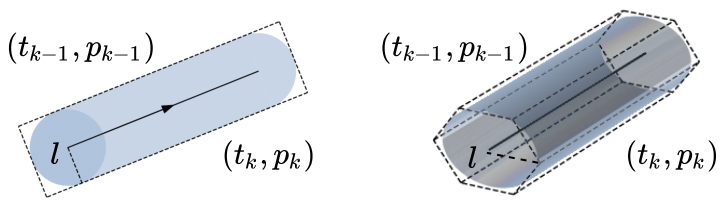
\includegraphics[width=0.8\columnwidth]{moving.png}
\caption{Examples of moving obstacles in 2D and 3D workspaces. All the possible swept area is in blue, and is over approximated to polytopes as shown with dashed line boundaries.}
\label{fig:moving}
\end{figure}

During replanning, some agents are treated as moving obstacles for other agents. Here we introduce our method for encoding the possible swept area of a path segment as a moving obstacle. Consider a segment from $(t_{k-1}, p_{k-1})$ to $(t_k, p_k)$. As we know all the swept area at position $p$ is $R = p \oplus B_{l}(0)$, we can calculate its moving obstacle as $(t_{k-1}, t_k, \texttt{Poly}(H_k, b_k)$), where $\texttt{Poly}(H_k, b_k)$ is a polygon containing all the possible swept area during duration $(t_{k-1}, t_k)$. Thus, if other agents do not swept $\texttt{Poly}(H_k, b_k)$ during $(t_{k-1}, t_k)$, their paths are guaranteed to be collision-free. The central axis of this moving obstacle is in the direction $\mbox{atan2}(p_{k} - p_{k-1})$ with length $2l + \norm{p_k - p_{k-1}}$. In a 2D workspace, the cross section of this tube is a line that is vertical to the central axis, and its width is $2l$. In a 3D workspace, the cross section is a circle with radius $l$. We further over approximate this circle as a polygon such as a octagon. Figure~\ref{fig:moving} shows examples in 2D and 3D workspace. 



%Even though PBS is incomplete in general, the recent results in PBS show it is a faster and near-optimal coordination method compared to complete conflict-based algorithms such as CBS~\cite{sharon2015conflict} and its variants. 
%Its high-level search follows the depth-first order to explore a priority tree whose nodes represent different (partial) priority orderings between agents. When it is faced with a collision, PBS chooses which agent should be given a higher priority and expands the tree. When a new priority is added, the low-level search of PBS finds an individually optimal path for lower-priority agents independently. When there is no solution in the current branch, the search backtracks and explores other branches until a collision-free solution is found.  



% \begin{algorithm}[t]\small
% \caption{\textsl{S2M2 Algorithm}}\label{alg:main}
% \KwIn{$\langle \mathcal{W}, O, \mathcal{A},\mathcal{X}^\texttt{init}, \mathcal{X}^\texttt{goal}, G \rangle$}
% \KwOut{$S = \{(\xi_{1,\texttt{ref}}, u_{1,\texttt{ref}}),..,(\xi_{N,\texttt{ref}}, u_{N,\texttt{ref}})\}$}
% \For{$\mathcal{A}_i \in \mathcal{A}$}
% {\tcp{$E_i = (e_{i,\texttt{max}}, T_{i,\texttt{min}}, T_{i,\texttt{min}}^\prime)$}
% $E_i \gets \textsl{ReachabilityEnvelope}(\mathcal{A}_i,\mathcal{X}^\texttt{init}_i,\mathcal{X}^\texttt{Goal}_i,g_i)$\;\label{alg:init_error}
% $S_i \gets \textsl{Replan}(\mathcal{W}, O, \{\}, \mathcal{A}_i, S^\texttt{init}_{i}, S^\texttt{goal}_{i}, RE_i)$\label{alg:init_path}\;}

% $Q \gets \{(S, \{\})\}$\;\label{alg:init_Q}
% \While{$Q \not = \{\}$}
% {$(S, \PREC) \gets 
% \text{ pop } Q$ \label{alg:pop}\;
% \lIf{$\textsl{CollisionFree}(S, \mathcal{A}, e_\text{max})$\label{alg:check_collision}}
% {\KwRet{$S$}}
% $(\mathcal{A}_i, \mathcal{A}_j) \gets \textsl{FirstCollidingPair}(S)$ \;
% \For{$(a \prec b) \in \{(i \prec j),  (j \prec i)\}$\label{alg:child}}
% {$\PREC' \gets \PREC \cup (a \prec b)$\;
% $S' \gets S$\;
% $S^H_b \gets \{S'_{r}| a_r \in \textsl{HigherPriorityAgents}(\PREC', b)\}$\;
% $O'_b \gets \textsl{MovingObstalces}(S^H_b, E^\texttt{max})$\;\label{alg:moving}
% $S'_b \gets \textsl{Replan}(\mathcal{W}, O, O'_b, \mathcal{A}_b, \mathcal{X}^\texttt{init}_{b}, \mathcal{X}^\texttt{goal}_{b}, E_b)$\;\label{alg:replan}
% \lIf{$S'_b \not = \{\}$}{$\text{push } (S', \PREC') \text{ to } Q$\label{alg:push}}}}
% \KwRet{$\{\}$}\label{alg:empty}

% \end{algorithm}






%S2M2 (Algorthm~\ref{alg:main}) takes as input workspace $\mathcal{W}$, obstacles $O$, agent models $\mathcal{A} = \{\mathcal{A}_i\}_i$, initial state sets $\mathcal{X}^\texttt{init}=\{\mathcal{X}^\texttt{init}_i\}_i$, goal sets $\mathcal{X}^\texttt{goal}=\{\mathcal{X}^\texttt{goal}_i\}_i$, and tracking controller for each agent $G = \{g_i\}_i$. The algorithm outputs a set of collision-free paths for all the agents or an empty set if the priority tree is exhausted. We first compute the maximum error $E^\texttt{max}_i$, minimum duration of the last segment $T^{\texttt{min},\prime}_i$, the minimum time duration to for each segment $T^\texttt{min}_i$ (Line~\ref{alg:init_error}). Then, we use this formation to plan paths for each agent individually (Line~\ref{alg:init_path}), which is an implementation of Section~\ref{section:approach:milp}. 
%S2M2 then performs PBS to coordinate agents and resolve collisions by exploring a priority tree (PT). PBS starts with the root PT node, which contains the initialized paths and an empty ordering (Line~\ref{alg:init_Q}). %The node with the least priority orders is expanded first, and thus follows the depth-first search. 


\section{Experimental Results}\label{section:results}

We present experimental results on both 2D and 3D environments with ground vehicles and quadrotor models, respectively.  We used DryVR \cite{fan2017d} to generate reachability envelopes and Gurobi 9.0.1 \cite{gurobi2020gurobi} as the MILP solver. We compared S2M2 with the state-of-the-art 2D planner ECBS-CT \cite{cohen2019optimal} and 3D planner MAPF/C+POST \cite{honig2018trajectory}. All experiments were run on a 3.40GHZ Intel Core i7-6700 CPU with 36GB RAM with a runtime limit of $100$s. We repeated each experiment 25 times for each agent number using randomly generated initial and goal locations for the agents. We report the average runtime, success rates (i.e., the percentages of solved instances within the runtime limit), and flowtime (i.e., makespan sum of all single-agent plans) for each agent number on each map. 


\begin{figure}[t]
  
    \centering
    \subfloat[Arena.]{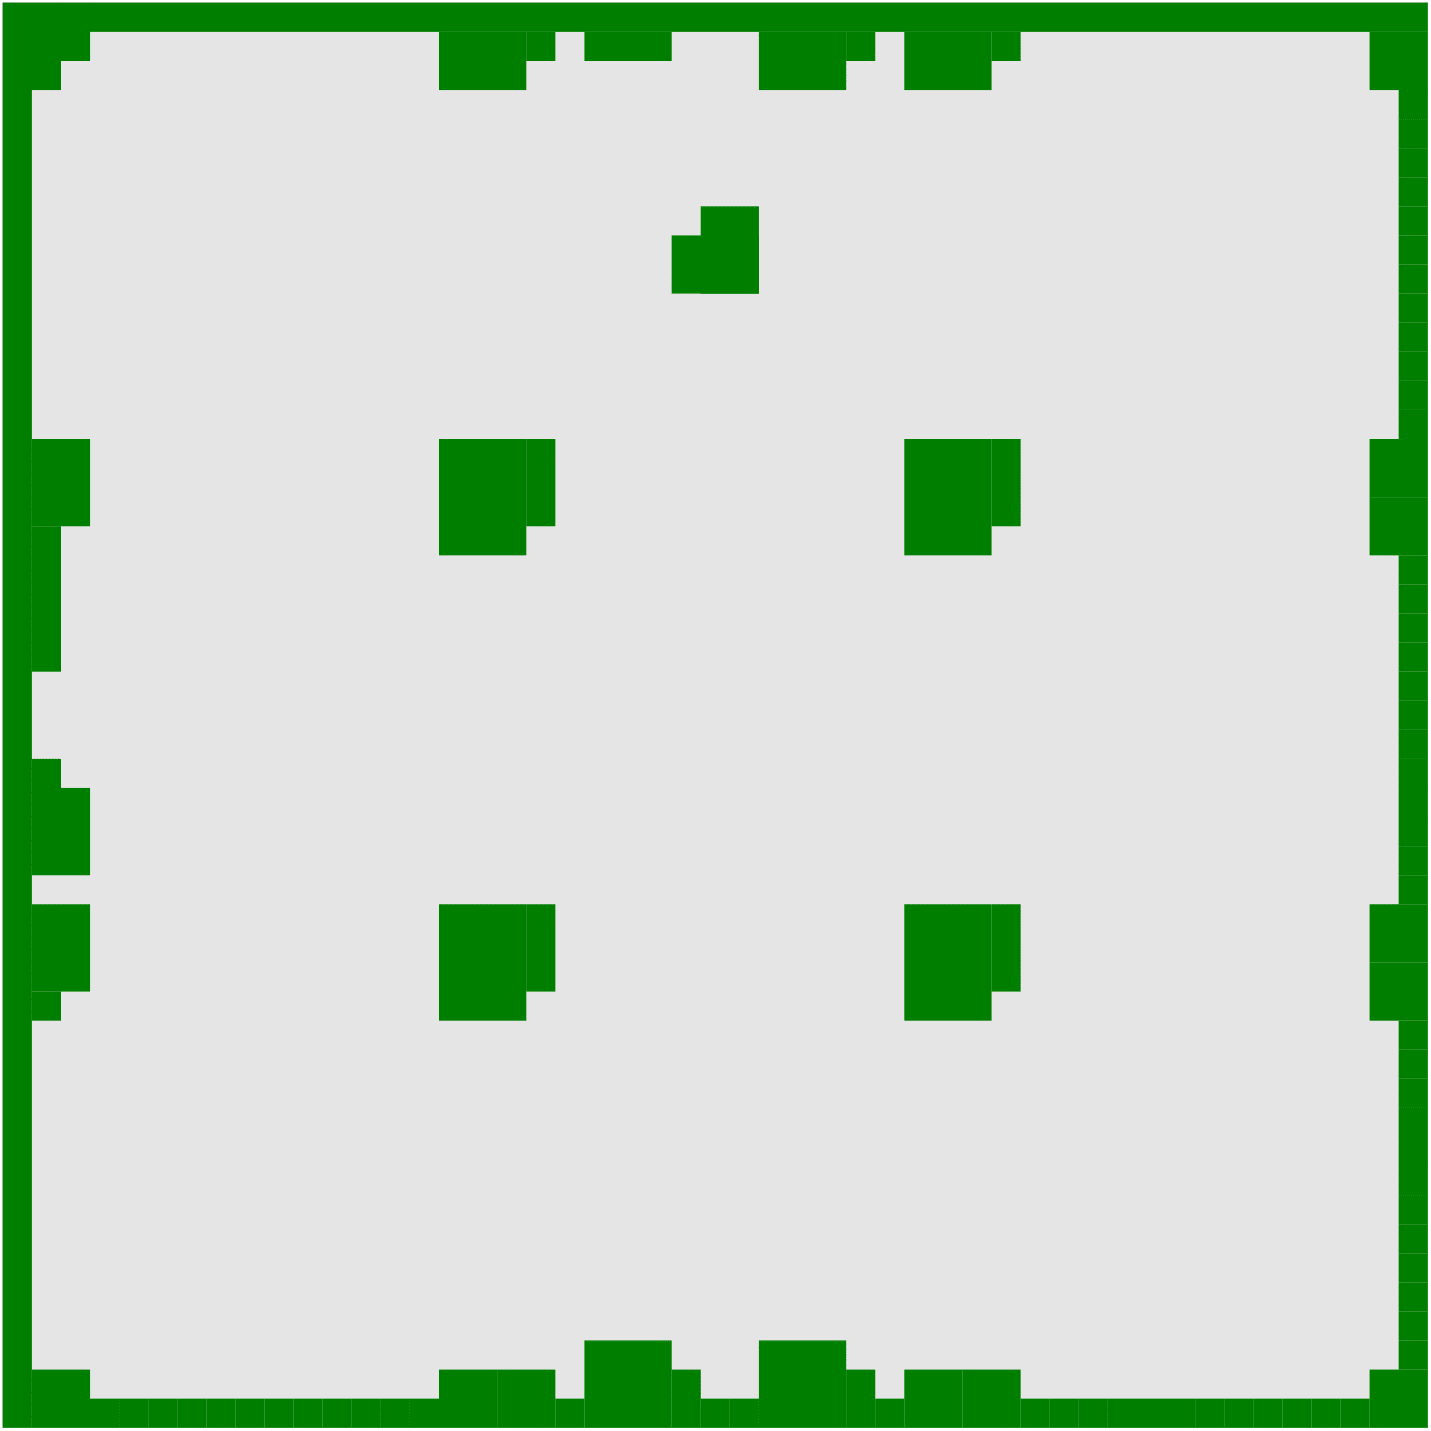
\includegraphics[width=0.2\columnwidth]{arena.png}}
    \,\,\,\,\,\,
    \subfloat[Den502d.]{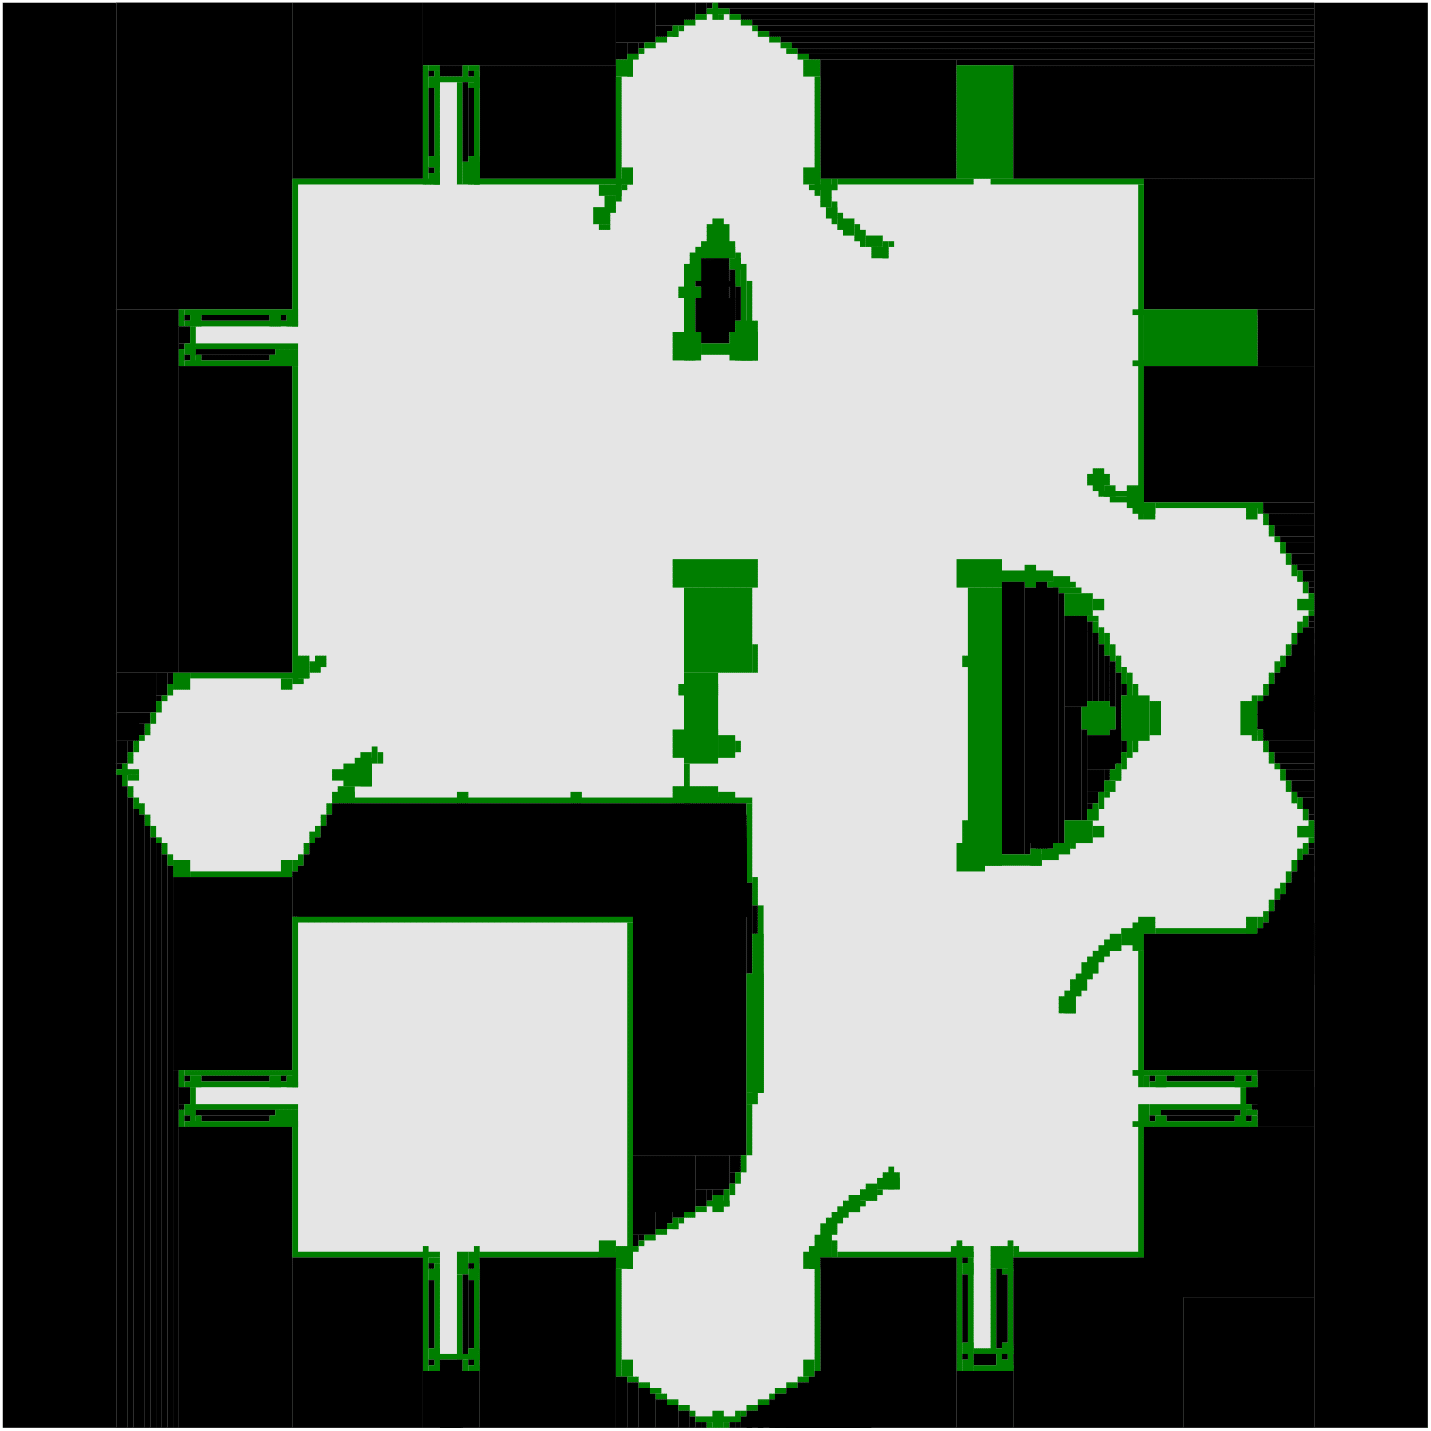
\includegraphics[width=0.2\columnwidth]{den502d.png}}
    \,\,\,\,\,\,
    \subfloat[Wall.]{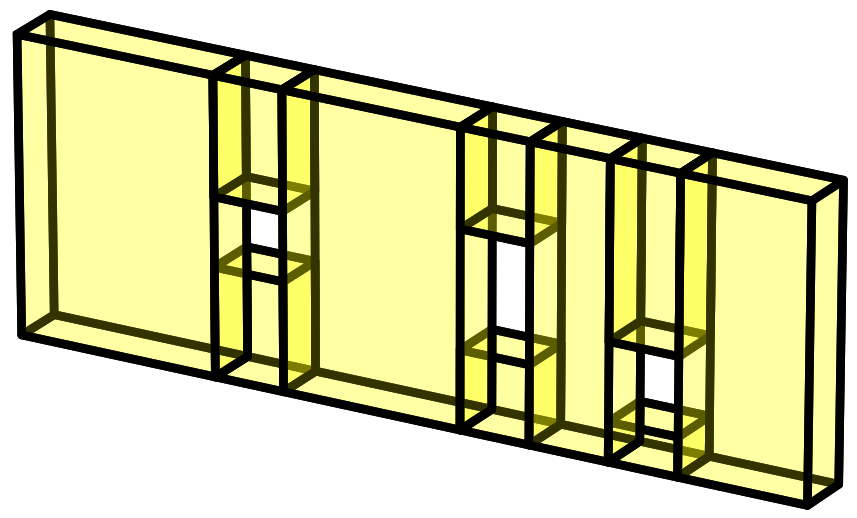
\includegraphics[width=0.28\columnwidth]{wall.png}}
    \caption{Maps and scenarios.}
    \label{fig:map}

\end{figure}

\subsubsection{2D Experiment}
We compare S2M2 against ECBS-CT on two benchmark maps from the Grid-Based Path Planning Competition (GPPC)\footnote{GPPC: https://movingai.com/GPPC}, namely Arena (49 $\times$ 49) and Den502d (251 $\times$ 211). % are representative of obstacles-rich environments. 
We assume a disc-shaped agent with a radius of $0.5$. While agent dynamics for ECBS-CT is approximated with sixteen discrete orientations and five primitives, which is taken from the Search-based Planning Laboratory (SBPL)\footnote{
SBPL: http://sbpl.net}, S2M2 considers a vehicle model with continuous, nonholonomic, nonlinear dynamics from \cite{rodriguez2014trajectory} with additional bounded disturbances.  The cost multiplier for the motion primitive model is set to $1$, which means no preferred action is specified. We set the maximum velocity in both planners to be $1$. We set the focal weight $\omega$ (i.e., suboptimality ratio) for ECBS-CT to $1.2$ and $1.5$. The average runtimes and success rates of our method and ECBS-CT on these two maps are given in Figure~\ref{fig:time}(a)-(d). The corresponding solution qualities are given in Table~\ref{table:cost}. Note that the pre-computation time is discussed separately and not added to the average runtime.

%The corresponding solution qualities are given in Table~\ref{table:cost}(a).
First of all, we observe that S2M2 is several magnitudes faster than ECBS-CT in terms of the pre-processing time. While S2M2 takes $0.33s$ to pre-compute the spatial error bound and the minimum duration for all agents, the time for ECBS-CT to pre-compute the heuristic is $0.27s$ on Arena and $18.18s$ on Den502d for each agent, which makes the total pre-processing time for ECBS-CT very large. For example, for each instance on Den502d with 60 agents, ECBS-CT spends roughly $1,100s$ to compute these heuristics. 

Furthermore, S2M2 outperforms ECBS-CT in terms of both runtimes and success rates, % even we set the focal weight of ECBS-CT to $1.5$, 
as shown in Figure~\ref{fig:time}(a)-(d). While S2M2 halves the runtime of ECBS-CT on Arena for most instances when $\omega = 1.5$, it is roughly one-third of that when $\omega = 1.2$ (Figure~\ref{fig:time}(a)). In Figure~\ref{fig:time}(c), the runtime of ECBS-CT does not change much with different weights on Den502d. While S2M2 takes half the time than ECBS-CT for most Den502d instances, S2M2 is one magnitude faster when the agent number is less than $40$. As shown in Figure~\ref{fig:time}(b)(d), the success rates of ECBS-CT drop much faster than S2M2. When ECBS-CT fails half the instances, S2M2 still solves more than $90\%$ of them. We do not include the case when $\omega = 1$ (i.e., search for optimal solutions) since ECBS-CT merely solves instances even for $10$ agents. We also test with larger focal weights, but it does not show significant improvement over runtimes or success rates.

In Table~\ref{table:cost}, we can see S2M2 reduces at least half the flowtime for Arena instances, and this reduction is up to $70\%$ as the agent number increases. This is because S2M2 directly plans high-fidelity models on a continuous map over continuous timeline, which provides more flexibility in avoiding collisions, especially in smaller maps. On the larger map Den502d, we can still observe roughly $15\%$ cost reduction.  

\begin{figure}[t]
    % \vspace{4pt}
    \centering
    \subfloat[Runtimes for Arena.]{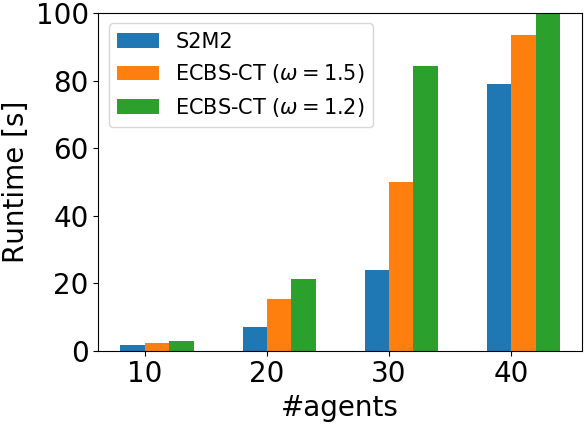
\includegraphics[width=0.48\columnwidth]{arena_time.png}}
    \,
    \subfloat[Success rates for Arena.]{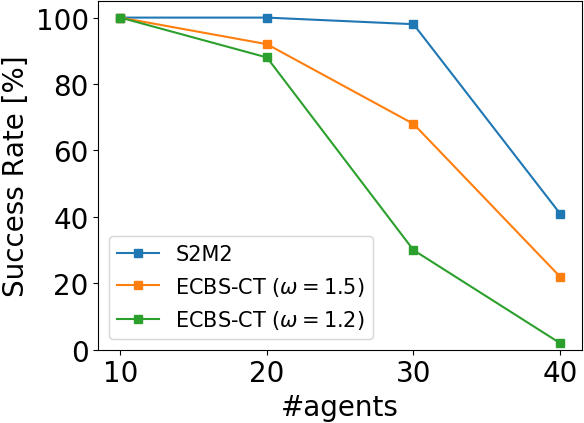
\includegraphics[width=0.48\columnwidth]{arena_success.png}}
    \,
    \subfloat[Runtimes for Den502d.]{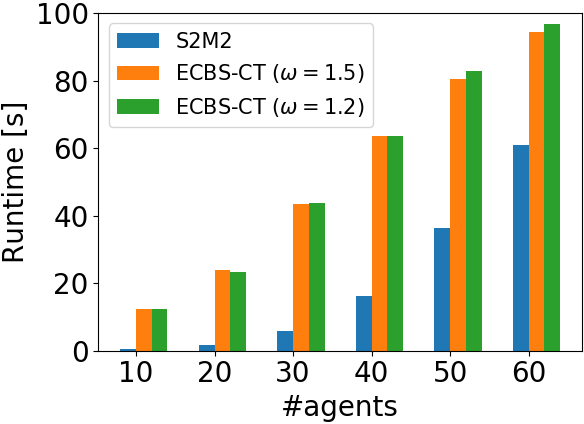
\includegraphics[width=0.48\columnwidth]{den502d_time.png}}
    \,
    \subfloat[Success rates for Den502d.]{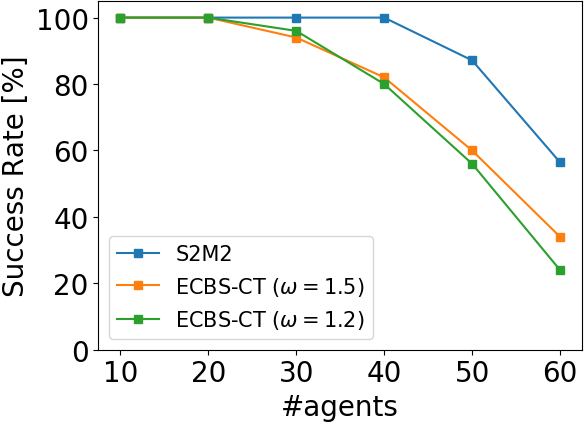
\includegraphics[width=0.48\columnwidth]{den502d_success.png}}
    \,
    \subfloat[Runtimes for Wall.]{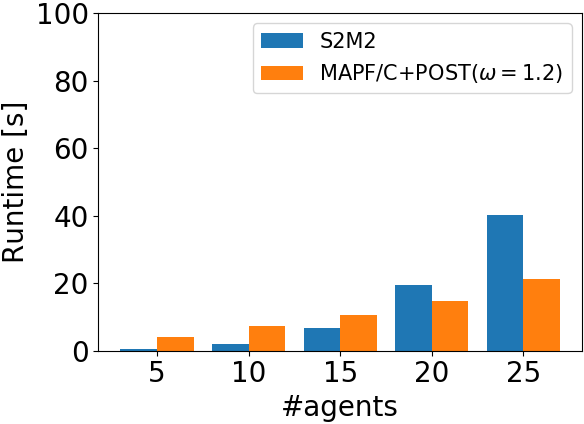
\includegraphics[width=0.48\columnwidth]{wall_time.png}}\
    \,
    \subfloat[Success rates for Wall.]{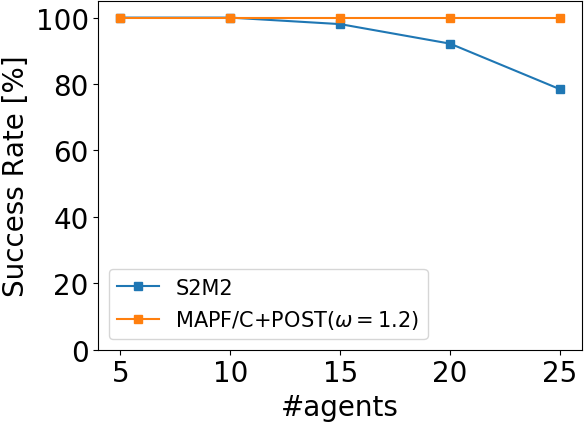
\includegraphics[width=0.48\columnwidth]{wall_success.png}}
    \caption{Runtimes and success rates.}
    \label{fig:time}
\end{figure}



\begin{table}[t]\scriptsize
\centering

% \subfloat[Solution quality for Arena and Den502d.]{
% \begin{tabular}{|c|c||c|c|c|}
% \hline
%  & \#agents & S2M2  & \makecell{ECBS-CT \\ ($\omega=1.2$)} & \makecell{ECBS-CT \\ ($\omega=1.5$)}  \\ \hhline{|=|=||=|=|=|}
% \multirow{5}{*}{\rotatebox[origin=c]{90}{\centering Arena}} 
% & 10 & 382.02 & 867.83 & 868.00  \\ \cline{2-5} 
% & 20 & 741.20 & 1848.07 & 1948.07 \\ \cline{2-5} 
% & 30 & 1062.60 & 2929.95 & 3147.36 \\ \cline{2-5} 
% & 40 & 1366.23 & NA & 4554.60 \\ \hhline{|=|=||=|=|=|}

% \multirow{5}{*}{\rotatebox[origin=c]{90}{\centering Den502d}}
% & 10 & 1292.01 & 1566.78 & 1567.87 \\ \cline{2-5} 
% & 20 & 2569.11 & 3135.57 & 3134.96 \\ \cline{2-5} 
% & 30 & 3962.72 & 4621.11 & 4620.03 \\ \cline{2-5} 
% & 40 & 5517.90 & 6292.29 & 6202.304 \\ \cline{2-5} 
% & 50 & 7289.37 & 7798.79 & 7821.35 \\ \cline{2-5} 
% & 60 & 8681.73 & 9452.26 & 9480.53 \\ \hline
% \end{tabular}}

% \subfloat[Solution quality for Wall.]{

% \begin{tabular}{|c|c||c|c|c|}
% \hline
%  & \#agents & S2M2  & \makecell{MAPF/C} & \makecell{MAPF/C + POST}  \\ \hhline{|=|=||=|=|=|}
% \multirow{5}{*}{\rotatebox[origin=c]{90}{\centering Wall}} 
% & 5 & 48.00 & 50.32 & 80.35  \\ \cline{2-5} 
% & 10 & 102.77 & 103.08 & 142.27  \\ \cline{2-5} 
% & 15 & 162.37 & 152.38 & 200.36 \\ \cline{2-5} 
% & 20 & 230.75 & 200.67 & 230.00 \\ \cline{2-5} 
% & 25 & 299.29 & 265.09 & 315.20  \\ \hline
% \end{tabular}

% }
{
\begin{tabular}{|c|c||c|c|c|}
\hline
 & \#agents & S2M2  & \makecell{ECBS-CT \\ ($\omega=1.2$)} & \makecell{ECBS-CT \\ ($\omega=1.5$)}  \\ \hhline{|=|=||=|=|=|}
\multirow{5}{*}{\rotatebox[origin=c]{90}{\centering Arena}} 
& 10 & 382.02 & 867.83 & 868.00  \\ \cline{2-5} 
& 20 & 741.20 & 1848.07 & 1948.07 \\ \cline{2-5} 
& 30 & 1062.60 & 2929.95 & 3147.36 \\ \cline{2-5} 
& 40 & 1366.23 & NA & 4554.60 \\ \hhline{|=|=||=|=|=|}
\multirow{5}{*}{\rotatebox[origin=c]{90}{\centering Den502d}}
& 10 & 1292.01 & 1566.78 & 1567.87 \\ \cline{2-5} 
& 20 & 2569.11 & 3135.57 & 3134.96 \\ \cline{2-5} 
& 30 & 3962.72 & 4621.11 & 4620.03 \\ \cline{2-5} 
& 40 & 5517.90 & 6202.30 & 6292.29 \\ \cline{2-5} 
& 50 & 7289.37 & 7798.79 & 7821.35 \\ \cline{2-5} 
& 60 & 8681.73 & 9452.26 & 9480.53 \\ \hline
\end{tabular}}

\vspace{4pt}

{
\begin{tabular}{|c|c||c|c|c|}
\hline
 & \#agents & S2M2  & \makecell{MAPF/C} & \makecell{MAPF/C+POST}  \\ \hhline{|=|=||=|=|=|}
\multirow{5}{*}{\rotatebox[origin=c]{90}{\centering Wall}} 
& 5 & 48.00 & 50.32 & 80.35  \\ \cline{2-5} 
& 10 & 102.77 & 103.08 & 142.27  \\ \cline{2-5} 
& 15 & 162.37 & 152.38 & 200.36 \\ \cline{2-5} 
& 20 & 230.75 & 200.67 & 230.00 \\ \cline{2-5} 
& 25 & 299.29 & 265.09 & 315.20  \\ \hline
\end{tabular}
}
\caption{Solution quality (i.e., average flowtime) for Arena and Den502d (above) and Wall (below).}
\label{table:cost}
\end{table}



% \begin{table}[t]\scriptsize
% \centering

% \subfloat[Solution quality for Arena and Den502d.]{
% \begin{tabular}{|c|c||c|c|c|}
% \hline
%  & \#agents & S2M2  & \makecell{ECBS-CT \\ ($\omega=1.2$)} & \makecell{ECBS-CT \\ ($\omega=1.5$)}  \\ \hhline{|=|=||=|=|=|}
% \multirow{5}{*}{\rotatebox[origin=c]{90}{\centering Arena}} 
% & 10 & 382.02 & 867.83 & 868.00  \\ \cline{2-5} 
% & 20 & 741.20 & 1848.07 & 1948.07 \\ \cline{2-5} 
% & 30 & 1062.60 & 2929.95 & 3147.36 \\ \cline{2-5} 
% & 40 & 1366.23 & NA & 4554.60 \\ \cline{2-5} 
% & 50 & 1839.42 & NA &  NA \\ \hhline{|=|=||=|=|=|}

% \multirow{5}{*}{\rotatebox[origin=c]{90}{\centering Den502d}}
% & 10 & 1292.01 & 1566.78 & 1567.87 \\ \cline{2-5} 
% & 20 & 2569.11 & 3135.57 & 3134.96 \\ \cline{2-5} 
% & 30 & 3962.72 & 4621.11 & 4620.03 \\ \cline{2-5} 
% & 40 & 5517.90 & 6292.29 & 6202.304 \\ \cline{2-5} 
% & 50 & 7289.37 & 7798.79 & 7821.35 \\ \cline{2-5} 
% & 60 & 8681.73 & 9452.26 & 9480.53\\ \cline{2-5} 
% & 70 & 9408.21 & 11006.10 & 11028.50 \\ \hline
% \end{tabular}}

% \subfloat[Solution quality for Wall.]{

% \begin{tabular}{|c|c||c|c|c|}
% \hline
%  & \#agents & S2M2  & \makecell{MAPF/C} & \makecell{MAPF/C + POST}  \\ \hhline{|=|=||=|=|=|}
% \multirow{5}{*}{\rotatebox[origin=c]{90}{\centering Wall}} 
% & 5 & 48.00 & 50.32 & 80.35  \\ \cline{2-5} 
% & 10 & 102.77 & 103.08 & 142.27  \\ \cline{2-5} 
% & 15 & 162.37 & 152.38 & 200.36 \\ \cline{2-5} 
% & 20 & 230.75 & 200.67 & 230.00 \\ \cline{2-5} 
% & 25 & 299.29 & 265.09 & 315.20   \\ \cline{2-5} 
% & 30 & 365.62 & 331.11 & 375.58 \\ \hline
% \end{tabular}

% }
% \caption{Solution quality (i.e., average flowtime) results.}
% \label{table:cost}
% \end{table}

\subsubsection{3D Experiment}
We use map Wall ($13 \times 13 \times 5$) from \cite{honig2018trajectory}.  In this scenario, a nano-quadrotor team \cite{preiss2017crazyswarm} starts from one side of the wall with three windows and is asked to fly to the other side. We compare S2M2 with MAPF/C+POST \cite{honig2018trajectory}, which performs a generalized-MAPF algorithm called MAPF/C on a graph with sparse samples and then post-processes the discrete solution to valid continuous trajectories. We set the maximum velocity in both planners to be $1$. We use the same parameters for sampling and post-processing as the original paper. The focal weight of MAPF/C is chosen to be $1.2$. In post-processing, we set the total iterations to $7$ and continuity degree to $4$. The average runtime and success rate of our method and MAPF/C+POST are given in Figure~\ref{fig:time}(e)-(f) while the solution qualities are given in Table~\ref{table:cost}.

While it takes $0.83s$ for S2M2 to pre-compute the error bound and minimum duration, the time to sample and annotate roadmaps for MAPF/C+POST is $1570.94s$ in total. Its sampling and annotating procedures, which are critical to its efficiency and solution qualities, take such long because they require computationally expensive distance checking on all edge pairs. Thus, MAPF/C+POST is sensitive to the map size and only scales to small maps. We also tested its sampling module with the 3D Arena map ($49 \times 49 \times 5$) and failed to get a reasonably connected roadmap in hours. 

%which are $0.092$ and $1.10s$,

Although MAPF/C+POST is efficient on sparse, well-connected roadmaps, S2M2 can still solve most instances faster when \#agents $<20$. The runtime is less than $1$s for instances with $10$ agents. In Table~\ref{table:cost}, we also observe that S2M2 has up to $40\%$ cost reduction compared to MAPF/C+POST trajectories. Even though the discrete MAPF/C solution is bounded suboptimal, %MAPF/C uses an approximated model without considering dynamics, and thus 
the quality of its valid continuous trajectory is not guaranteed.

\section{Conclusions}
We presented S2M2, a fast and effective multi-agent motion planner that generates provably safe plans for agent models with high-dimensional, nonlinear dynamics and bounded disturbances. S2M2 plans piecewise linear paths that satisfy certain safe bounds and coordinates multiple agents using the priority-based search. We show that S2M2 improves both the solving time and the solution quality compared to two state-of-the-art multi-agent motion planners. Especially, S2M2 saves much time on pre-processing.

\section*{Acknowledgements}
This work at Massachusetts Institute of Technology was supported by Kawasaki Heavy Industries, Ltd (KHI) under grant number 030118-00001. This article solely reflects the opinions and conclusions of its authors and not KHI or any other Kawasaki entity.
\bibliography{bib}
\end{document}

% \subsection{Coordinate Agents by Adjusting Paths}\label{section:approach:adjust}

% Given a path, we can divide some segments into multiple segments and obtain different paths. The new paths can be instantiated to different reference trajectories in which the agent follows the previous heading direction at each position but with different velocities. This flexibility in adjusting agent speeds without replanning renders a cost-effective way to coordinate multiple vehicles. 

% When checking the collision between multiple agents given their paths, we first check whether these paths are collided by assuming a constant position change rate during each segment. We say the trajectories of two different agents are colliding if the distance of their positions is less than $l + l'$ at some time, where $l$ and $l'$ are the maximum radius of their reaching areas. If they are collision-free, we succeed in finding a valid reference trajectories for each agent; otherwise, we identify all the pairs of colliding segments $C = \{(s_{ik}, s_{i'k'})\}$ and $s_{ik}$ refers to the $k^\text{th}$ segment of agent $a_i$. We further denote the involved agents as $\mathcal{A}^c$ and all the involved segments as $S^c$. Then, we try resolving them by adjusting their speeds by dividing some segments into multiple segments. We repeat dividing segments until collision-free paths are found, or no valid dividing plan can be found.

% For a line segment $s_{ik}$ starting from $p_{i(k-1)}$ at time $t_{i(k-1)}$ and ending at $p_{ik}$ at time $t_{ik}$, the agent velocity can vary as long as the agent can complete the segment right on time. We divide each segment $s_{ik}$ into $N$ consecutive segments with the same heading direction and the $n^\text{th}$ segment is denoted as $s_{ikn}$, where $N T_\text{min} <= t_{ik} - t_{i(k-1)}$ and $T_\text{min}$ is the least duration for each segment. We use variables $[t_{ik(n-1)}, t_{ikn}]$ with continuous domain $[t_{i(k-1)}, t_{ik}]$ to represent the start and end times of $s_{ikn}$, and the positions at the start and end times are $p_{ik(n-1)}$ and $p_{ikn}$. To ensure all the segments can be completed right on time, we have the constraints:

% \begin{equation}
%     \begin{aligned}
%       (p_{ik0} = p_{i(k-1)}) \land (t_{ik0} = t_{i(k-1)}) \\
%       (p_{ikN} = p_{ik)}) \land (t_{ikN} = t_{ik})
%       \ \forall s_{ik} \in S^c
%     \end{aligned}
% \end{equation}

% We also has an intermediate variable $\lambda_{ikn}$ with continuous domain $(0, 1)$ to represent the ratio of length of the segment $s_{ikn}$ over that of $s_{ik}$. As the system dynamics should respected, we have the following constraints:

% \begin{equation}
%     \begin{aligned}
%         p_{ikn} - p_{ik(n-1)))} = (p_{ik} - p_{i(k-1)})\lambda_{ikn}  \\
%         H_{p}(p_{ikn} - p_{ik(n-1)}) \leq   b_{p}(t_{ikn} - t_{ik(n-1)}) \\
%       \forall s_{ik} \in S^c, \forall n \in \{1,2,..,N\}
%     \end{aligned}
% \end{equation}

% To obtain collision-free paths, we require two pairs of segments of different agents should be either disjoint over time or space. We add the following constraints:
% \begin{equation}\small
%   \begin{aligned}
%     (H_{ii'kk'}p_{ik(n-1)} > b_{ii'kk'} - M\alpha_{iki'k'}) \\
%     \land (H_{ii'kk'}p_{ikn} > b_{ii'kk''} - M\alpha_{iki'k'}) \\
%     \land (t_{ikn} < t_{i'k'(n'-1)} + M \alpha_{iki'k', <}) \\ 
%     \land (t_{i'k'n'} < t_{ik(n-1)} + M \alpha_{iki'k', >})\\ 
%     \land ((\sum_{j=1}^{\texttt{dP}(H_{ii'kk'})} \alpha^{(j)}_{ii'kk'}) + \alpha_{iki'k', <} + \alpha_{iki'k', >} \\ \leq  \texttt{dp}(H_{ii'kk'}) + 1) \\
%      \forall (s_{ik}, s_{i'k'}) \in C , \forall n \in \{1,2,..N\}, \forall n' \in \{1,2,..,N'\},
%   \end{aligned}
% \end{equation}
% where $\texttt{Poly}(H_{ii'kk'}, b_{ii'kk'})$ is a polytope  over approximation of ball $B_{(l_{ik}+l_{i'k'})}(0)$ in the workspace, and $l_{ik}$ and $l_{i'k'}$ are sweping area radius of agents $a_i$ and $a_{i'}$ at segment $k$ and $k'$, respectively.
